\documentclass[10pt]{article}

\usepackage[letterpaper,textwidth=5.5in,textheight=9in,top=1in]{geometry}
\usepackage[T1]{fontenc}
\usepackage[utf8]{inputenc}
\usepackage{amsmath}
\usepackage{newtxtext}
\usepackage{newtxmath}
\usepackage{inconsolata}
\usepackage{microtype}
\usepackage{booktabs}
\usepackage{graphicx}
\usepackage{enumitem}
\setlist{noitemsep, topsep=2pt}
\usepackage[round]{natbib}
\PassOptionsToPackage{hyphens}{url}
\usepackage{hyperref}
\usepackage[capitalise,sort]{cleveref}
\usepackage{algorithm}
\usepackage{algpseudocode}
\usepackage{placeins}
\usepackage{tikz}
\usetikzlibrary{positioning,fit,calc,backgrounds,arrows.meta}
\crefname{algorithm}{Algorithm}{Algorithms}
\crefname{figure}{Figure}{Figures}
\crefname{table}{Table}{Tables}

% Notation macros: define each recurring symbol once so usage stays consistent.

% Seed-intervention scores
\newcommand{\phicf}{\phi_{\mathrm{cf}}}      % counterfactual faithfulness
\newcommand{\phisup}{\phi_{\mathrm{sup}}}    % positive-context suppression

% Sets and spaces
\newcommand{\R}{\mathbb{R}}                  % the reals
\newcommand{\posset}{\mathcal{P}_f}          % stored positive contexts of seed f
\newcommand{\negset}{\mathcal{N}_f}          % contrast (negative) contexts of seed f

% Discovery objective and attributions
\newcommand{\Lcf}{\mathcal{L}^{\mathrm{cf}}} % counterfactual gap objective
\newcommand{\Scf}{S_g^{\mathrm{cf}}}         % counterfactual attribution of upstream latent g
\newcommand{\Sab}{S_g^{\mathrm{ab}}}         % ablation attribution of upstream latent g
\newcommand{\preact}{\hat{a}_f}              % seed encoder pre-activation


% Abstract set as in the NeurIPS/ICLR styles: \large centred heading, body at
% full 10pt, side-indented 3pc each side (their styles set \leftmargini=3pc,
% wider than article.cls's 2.5em default).
\renewenvironment{abstract}{%
  \vskip .075in%
  \centerline{\large\bfseries\abstractname}%
  \vspace{0.5ex}%
  \list{}{\leftmargin 3pc \rightmargin \leftmargin}%
  \item\relax
}{\endlist\vskip 1ex}

\graphicspath{{figures/}}

\title{%
  \vspace*{-2.5em}%
  \rule{\linewidth}{4pt}\\[0.4em]
  \bfseries What Makes a Feature Fire? \\ Discovering Signed Causal Dependencies Between \\ Sparse Autoencoder Latents\\[0.1em]
  \rule{\linewidth}{0.7pt}%
}
\author{%
  \textbf{Daniel Davies}\thanks{Correspondence to \texttt{danieljamesdavies12@gmail.com}.} \\ Independent
  \and
  \textbf{Dr Weibo Liu} \\ Brunel University London
}
\date{}

\begin{document}

% =============================================================================
% V2 REWRITE IN PROGRESS (2026-07-30) — see paper/rewrite-tracker.md for the
% step plan and paper/paper-updates.md for the change specifications.
% v1 is backed up at paper/backup-2026-07-30-pre-rewrite/.
% Placeholder subsections are intentional: they are the agreed target skeleton.
% =============================================================================

\maketitle

% STEP 2 DONE (2026-07-30). Numbers vintage: the ~16% membership-churn figure is
% B6l (solid, bit-determinism established); the drivers/closure magnitudes are
% deliberately qualitative pending the depth-stratified rerun.
\begin{abstract}
Circuit discovery methods in mechanistic interpretability typically select a behavioural or logit-level endpoint and identify the features contributing to it.
But a model's outputs are filtered summaries of its computation.
This paper instead treats an internal sparse feature as the target of explanation: given a seed sparse autoencoder (SAE) latent in TuringLLM, we ask what makes it fire.
Discovery combines contrastive gradient attribution through the seed's encoder pre-activation --- defined and differentiable even where the seed is silent --- with a learned-mask method that frames latent-endpoint discovery as an optimization problem, and every discovered dependency is validated by intervention on the seed itself.
The resulting picture separates along the two criteria the word ``circuit'' conflates.
\emph{Interventional control} is concentrated: a compact signed circuit of activators, inhibitors, and supports suffices to impose the seed's activation.
\emph{Faithfulness} --- the circuit alone reproducing the seed, with everything else ablated --- is collective, position-local, and depth-scaled: it requires orders of magnitude more members, individually at the measurement floor, whose collective removal silences the seed.
That cost is indexed by amplitude semantics: granting each member a learned scalar amplitude collapses the faithful membership by one to two orders of magnitude --- a compact weighted circuit passes both criteria --- and survives a matched null in which random same-size sets receive identically fitted amplitudes and fail on every draw.
Which latents make the cut is partly underdetermined --- perturbations as small as float rounding exchange roughly 16\% of members at unchanged circuit quality --- so we report memberships as size-calibrated families rather than unique sets.
Behaviour-endpoint circuits, run under matched conditions, exert no control over whether an internal latent fires, and vice versa: the two questions are complementary, not reducible.
Requiring no behavioural task, the pipeline runs across the full SAE bank.
\end{abstract}

\section{Introduction}
% STEP 2 DONE (2026-07-30): 2x2 recast replaces the falsifiable absolute claim;
% six-contribution list per the portfolio revision.

We can watch what a language model produces, but we cannot yet trace how it arrives there.
Individual neurons are largely uninformative: models pack more features than they have dimensions, exploiting high-dimensional geometry through superposition~\citep{elhage2022toy}, so most neurons respond to incoherent mixtures of unrelated inputs.
Sparse autoencoders (SAEs) offer a way out, decomposing each dense activation vector into a handful of active latent features that tend to correspond to coherent semantic or syntactic patterns~\citep{cunningham2024sparse, bricken2023monosemanticity, gao2024scaling, templeton2024scaling}.

But individual latents are only the beginning of an explanation.
Knowing that a feature responds to mathematical notation is interesting; knowing which other features it recruits, suppresses, or depends on is where the mechanistic story lives.
Circuit discovery pursues that story, and its methods overwhelmingly root the explanation at an output-level endpoint: a logit, a probability, a behavioural metric.
This holds whether the nodes are architectural components~\citep{conmy2023towards, syed2023attribution} or sparse features~\citep{marks2025sparse, ameisen2025circuit}, and whether the circuit is found by search, attribution, or learned optimization~\citep{bhaskar2024finding, kharlapenko2025scaling}.
This is a powerful framing, but it is bounded by the endpoints we can name: a model computes many internal variables that never surface cleanly as any single behaviour, and an output-rooted graph reaches only the internal variables that project onto its chosen endpoint.
The internal endpoint itself has been approached, but only by thresholded attribution: methods that trace upstream of a chosen SAE feature attribute on prompts where the feature already fires, and validate none of the discovered dependencies by intervention~\citep{ge2024automatically}.
The remaining cell of this grid --- a circuit \emph{optimised} for a single internal feature's activation, and tested by intervening on that feature --- is, to our knowledge, empty.
It is where this paper works (\cref{fig:overview}).

\begin{figure}[t]
\centering
\begin{tikzpicture}[
  font=\scriptsize,
  panel/.style={draw=black!50, rounded corners=3pt, fill=black!2, inner sep=5pt},
  meth/.style={draw=black!55, rounded corners=2pt, align=center, fill=blue!7, inner sep=4pt, text width=2.85cm},
  arrow/.style={-{Stealth[length=1.8mm]}, black!60, thick},
  head/.style={font=\scriptsize\bfseries}
]
% ---------------- Panel A: the instance ----------------
\draw[panel] (-0.25,-2.35) rectangle (2.75,2.1);
\node[head] at (1.25,1.85) {any latent in the bank};
\foreach \i in {0,...,6} \foreach \j in {0,...,3}
  \fill[black!25] (0.30+\i*0.28, 0.45+\j*0.28) circle (0.040);
\fill[orange!90!black] (0.30+4*0.28, 0.45+2*0.28) circle (0.075);
\node[font=\scriptsize, orange!75!black] at (0.30+4*0.28+0.24, 0.45+2*0.28+0.20) {$f$};
\node[font=\tiny, black!60] at (1.25,0.13) {36 sites $\times$ 40{,}960 latents (\S\ref{sec:setting})};
% probes
\node[font=\scriptsize, anchor=west] at (0.05,-0.40) {probe contexts $\mathcal{D}_f$ (\S\ref{sec:evidence}):};
\draw[fill=green!14, draw=black!40] (0.15,-1.00) rectangle (1.35,-0.70);
\fill[green!55!black] (1.02,-1.00) rectangle (1.13,-0.70);
\node[font=\tiny, anchor=west] at (1.45,-0.85) {$f$ fires};
\draw[fill=black!8, draw=black!40] (0.15,-1.60) rectangle (1.35,-1.30);
\node[font=\tiny, anchor=west] at (1.45,-1.45) {$f$ silent};
\node[font=\tiny, black!60, anchor=west] at (0.05,-2.05) {+ ablation semantics $\pi$ \ (\S\ref{sec:problem})};
% ---------------- instance arrow ----------------
\node[font=\tiny, black!60] at (3.42,0.62) {$(f, \mathcal{D}_f, \pi)$};
\draw[arrow] (2.85,0.0) -- (4.25,0.55);
\draw[arrow] (2.85,-0.2) -- (4.25,-1.15);
% ---------------- Panel B: discovery ----------------
\node[meth] (attr) at (5.85,0.95)
  {\textbf{gradient attribution}\\ score every upstream latent\\ through the pre-activation;\\ rank and cut \ (\S\ref{sec:cfgrad}--\ref{sec:modes})\\[0.38cm]\mbox{}};
% rank-and-cut glyph: signed scores, threshold, dropped tail
\foreach [count=\i from 0] \h/\c in {0.30/blue!60!black!70, 0.24/red!65, 0.19/blue!60!black!70, 0.13/black!22, 0.09/black!22, 0.06/black!22}
  \fill[\c] ($(attr.south)+(-0.50+\i*0.17,0.10)$) rectangle ++(0.11,\h);
\draw[dashed, black!55] ($(attr.south)+(-0.01,0.05)$) -- ++(0,0.42);
\node[meth] (mask) at (5.85,-1.30)
  {\textbf{learned mask}\\ a gate per upstream latent;\\ relaxation of \cref{eq:p2star} \ (\S\ref{sec:ablmask})\\[0.36cm]\mbox{}};
% gate glyph: memberships harden open/closed around the threshold
\foreach [count=\i from 0] \c in {blue!60!black!85, blue!60!black!60, blue!60!black!40, black!18, black!12, black!8}
  \fill[\c] ($(mask.south)+(-0.44+\i*0.17,0.18)$) circle (0.058);
\draw[dashed, black!55] ($(mask.south)+(-0.015,0.02)$) -- ++(0,0.32);
% ---------------- Panel C: the two objects ----------------
\draw[panel] (7.85,-2.35) rectangle (13.65,2.1);
\node[head] at (10.75,1.85) {one seed, two criteria (\S\ref{sec:problem})};
% driver circuit (P1)
\foreach \y/\s in {1.45/$+$, 1.00/$-$, 0.55/$+$} {
  \draw[black!55, fill=blue!10] (8.18,\y) circle (0.11);
  \node[font=\tiny] at (8.18,\y) {\s};
  \draw[arrow] (8.31,\y) -- (9.02,1.00);
}
\fill[orange!90!black] (9.14,1.00) circle (0.10);
\node[font=\tiny, orange!75!black] at (9.14,1.28) {$f$};
\node[font=\scriptsize, align=left, anchor=west] at (9.45,1.05)
  {\textbf{interventional control --- (P1)}\\ signed, $10^{2}$--$10^{3}$:\\ inject where silent ($\phicf$),\\ suppress where firing ($\phisup$)};
% closure membership (P2): a multi-site mesh sustaining f
\foreach \ya/\yb in {-2.05/-1.65, -1.65/-1.25} {
  \foreach \i in {0,...,5}
    \draw[black!14, line width=0.3pt] (8.05+\i*0.19,\ya) -- (8.24+\i*0.19,\yb);
  \foreach \i in {1,...,6}
    \draw[black!14, line width=0.3pt] (8.05+\i*0.19,\ya) -- (7.86+\i*0.19,\yb);
}
\foreach \i in {0,...,6}
  \draw[black!14, line width=0.3pt] (8.05+\i*0.19,-1.25) -- (8.62,-0.84);
\foreach \yy in {-2.05,-1.65,-1.25}
  \foreach \i in {0,...,6}
    \fill[black!45] (8.05+\i*0.19,\yy) circle (0.035);
\fill[orange!90!black] (8.62,-0.78) circle (0.09);
\node[font=\tiny, orange!75!black] at (8.88,-0.72) {$f$};
\node[font=\scriptsize, align=left, anchor=west] at (9.45,-1.20)
  {\textbf{ablation faithfulness --- (P2)}\\ collective, $10^{4}$--$10^{5}$, depth-scaled\\ free execution: members permitted,\\ not forced ($\phi^{\mathrm{free}}$)};
% ---------------- arrows discovery -> objects ----------------
\draw[arrow] (attr.east) -- (7.80,1.00);
\draw[arrow] (attr.east) -- (7.80,-0.90);
\draw[arrow] (mask.east) -- (7.80,-1.30);
\end{tikzpicture}
\caption{Overview.
For \emph{any} SAE latent $f$ --- no behavioural task --- a per-seed problem instance $(f, \mathcal{D}_f, \pi)$ is formed from stored contexts where the seed fires and retrieved contexts where it is silent (\S\ref{sec:problem}).
Discovery runs by gradient attribution (counterfactual and ablation objectives, ranked and cut) and by learned-mask optimization (a gate per upstream latent), and the discovered circuit is examined under the two criteria the word ``circuit'' conflates: \emph{interventional control} (P1), validated by intervening on the seed itself, and \emph{ablation faithfulness} \cref{eq:p2} --- the measured cost of the circuit reproducing the seed alone under free execution, spanning every upstream site.
Control is concentrated; faithfulness is collective, position-local, and depth-scaled (\S\ref{sec:drivers-closure}).}
\label{fig:overview}
\end{figure}

Given a seed SAE latent, we ask: which other latents can causally increase, suppress, or sustain its activation?
The answer depends on the exam, and the literature tends to conflate two exams under the single word ``circuit''.
\emph{Interventional control} asks for a signed dependency neighbourhood with three operationally distinct roles --- \emph{counterfactual activators}, \emph{inhibitors}, and \emph{ablation supports} --- discovered by gradient attribution under contrasting context regimes and validated by direct intervention on the seed's activation; a compact circuit passes it.
\emph{Faithfulness} --- the field's own criterion, instantiated at the latent endpoint --- asks that the circuit alone reproduce the seed's activation under free execution, with every non-member removed; far more latents must remain able to fire before a circuit passes that.
Keeping the two criteria apart turns the size of the faithful set from an embarrassment into a measurement --- circuit size, we will argue, measures computational structure, and is not a knob to minimise.
No externally specified behavioural task is required at any point, so the procedure applies to any latent in the SAE bank.

We make six contributions.
\begin{itemize}
\item \textbf{Latent-endpoint causal discovery, validated by intervention.}
Signed dependencies discovered by contrastive attribution on contexts where the seed is \emph{silent} --- through its pre-activation, so gradients survive the silence --- and validated by intervening on the seed in both directions; negative-context construction is a controlled variable, and random contrasts can beat semantically close hard negatives.
\item \textbf{A learned-mask method for the latent endpoint.}
Circuit discovery as optimization~\citep{bhaskar2024finding}, moved to a single latent: a pre-activation objective forced by Top-K censoring, a multi-floor loss training one membership under up to three ablation semantics jointly~\citep{miller2024transformer}, annealed binarisation, one-probe size calibration, and learned per-member amplitudes that return a \emph{weighted circuit}.
\item \textbf{The control/faithfulness decomposition.}
Pinned evaluation asks whether the \emph{right} latents were found; free evaluation asks whether the circuit \emph{reproduces the seed alone} --- different questions with different answers, and the instrument behind every other result.
\item \textbf{The central finding: faithfulness is collective, position-local, and depth-scaled --- at natural amplitudes.}
% Magnitudes kept qualitative pending the depth-stratified rerun (14-Jul vintage).
Interventional control concentrates; faithfulness needs orders of magnitude more members, individually at the measurement floor yet collectively load-bearing, with an irreducible core that grows with seed depth --- and learned amplitudes collapse that cost by one to two orders of magnitude, locating most of it in amplitude-compensable redundancy.
\item \textbf{An evaluation protocol, and a measurement about membership itself.}
Every score names its ablation semantics --- the choice can reorder method rankings --- and membership is partly underdetermined (float rounding exchanges ${\sim}16\%$ of members at unchanged quality), so memberships are reported as families, not sets.
\item \textbf{A controlled boundary with behaviour-endpoint discovery.}
With the attribution estimator held fixed~\citep{marks2025sparse}, circuits explaining a logit exert zero control over whether a chosen latent fires, and vice versa: latent-endpoint discovery is not reducible to behaviour-endpoint discovery --- a scope result, measured rather than asserted.
\end{itemize}
We release the pipeline, discovery methods, and analysis code at \href{https://github.com/DanielJamesDavies/turing-explorer-circuit-discovery}{\nolinkurl{github.com/DanielJamesDavies/turing-explorer-circuit-discovery}}.

\section{Related Work}
% STEP 3 DONE (2026-07-30): B6/B6b/B6c/B6q/B7 additions landed; absolute
% endpoint claim scoped to the enumerated methods; build-on tone throughout.

\paragraph{Circuit discovery.}
The circuits programme began with manual analysis of model components~\citep{olah2020zoom, wang2023interpretability}; ACDC~\citep{conmy2023towards} automated the search, and attribution patching replaced exhaustive intervention with gradient approximations~\citep{nanda2023attribution, syed2023attribution, kramar2024atp}.
Sparse feature circuits~\citep{marks2025sparse} moved the nodes to SAE features --- with error nodes keeping reconstruction residuals in the graph, position-indexed nodes on templatic data, and an unsupervised pipeline over clustered behaviours --- while transcoders~\citep{dunefsky2024transcoders} factorize MLP circuits and attribution graphs~\citep{ameisen2025circuit, lindsey2025biology} instantiate position-indexed graphs per prompt at production scale; gradient-times-activation scoring of SAE latents also appears in GradSAE~\citep{shu2025beyond} and, at dictionary-training time, in g-SAEs~\citep{olmo2025features}.
In all of these, the objective is anchored at an output-level endpoint, even when that endpoint is discovered automatically.

\paragraph{Circuit discovery as optimization.}
Edge Pruning~\citep{bhaskar2024finding} reframed the search as an optimization problem --- continuous masks learned by gradient descent, built on $L_0$-gate and continuous-sparsification machinery~\citep{louizos2018learning, savarese2020winning}, with sparsity targeting in place of a fixed penalty --- and \citet{kharlapenko2025scaling} bring the same move to masks over SAE latents.
In both, the training objective is behavioural: a KL divergence or logit difference against the full model.
Our learned mask (\cref{sec:ablmask}) adopts this framing and its gate machinery, and moves the objective to a single latent's pre-activation; its per-member amplitudes additionally re-weight \emph{kept} components, where learned-value ablation~\citep{li2024optimal} learns constants for removed ones.

\paragraph{Latent-endpoint attribution.}
The distinction this paper draws is not methodological ingredients --- gradients, patching, masks, and sparse dictionaries are common stock --- but the root of the explanation, and the internal root is not unexplored: \citet{ge2024automatically} extract the subgraph activating a chosen SAE feature by thresholded hierarchical attribution, and latent attribution at OpenAI traces upstream causes of a chosen latent for debugging~\citep{duprelatour2025debugging}.
Both attribute on prompts where the feature already fires and stop short of intervention; we add attribution where the feature is \emph{silent}, learned-mask discovery in place of thresholds, and intervention validation of every discovered dependency.

\paragraph{Position-aware circuits.}
Position handling divides prior work into three strategies, each right for its setting: position-indexed nodes on templatic data~\citep{marks2025sparse}, per-instance graphs built one prompt at a time~\citep{ameisen2025circuit}, and schema-aligned positions across variable-length examples~\citep{haklay2025position}.
Our membership sets keep the position axis with none of these commitments --- per-position selection unioned over each sequence's causal prefix --- for the setting none of the three targets: one reusable circuit over arbitrary non-templatic text (\cref{sec:membership}).

\paragraph{Ablation semantics and faithfulness metrics.}
What ``removing'' a feature means is itself an experimental choice: \citet{li2024optimal} organise zero, mean, resample, and counterfactual ablations and propose an optimal constant; \citet{miller2024transformer} show faithfulness is not robust to these choices --- ``the ablation partly determines the task'' --- and \citet{mueller2024missed} argues the corruption distribution defines the counterfactual being measured.
We treat this relativity as a design input: every score names its semantics (\cref{sec:eval}), and the multi-floor objective trains one membership under up to three semantics jointly (\cref{sec:ablmask}).

\paragraph{Negative and contrastive contexts.}
Retrieved non-activating examples appear in automated interpretability for explanation scoring~\citep{paulo2024automatically}; \citet{paulo2025evaluating} find evaluations collapse when negatives come from neighbouring features --- convergent with our random-beats-close result (\cref{sec:results}); and \citet{oneill2024sparse} design corrupted negatives for task-level circuit identification.
We use retrieved negatives for causal discovery rather than explanation scoring, and treat their construction as a controlled variable with measured consequences.

\paragraph{The SAE basis.}
Static structure among latents is well documented --- co-occurrence and decoder geometry reveal modularity~\citep{li2025geometry}, coactivation-derived components steer behaviour~\citep{deng2026coactivation}, meta-decompositions show latents are not atomic~\citep{leask2025canonical}, and Jacobian SAEs train adjacent dictionaries for sparse computation between them~\citep{farnik2025jacobian} --- but it is correlational, geometric, or weight-based, where the relationships discovered here are context-conditioned and intervention-tested (\cref{sec:coact-results}).
The basis itself is imperfect: reconstruction errors are pathological~\citep{gurnee2024pathological}, downstream utility is mixed~\citep{smith2025negative}, and units are not canonical~\citep{leask2025canonical}.
This conditions our claims --- reconstruction residuals stay as explicit anchors, evaluation intervenes on measured activations, and the SAE basis is treated as a useful but imperfect sample of the model's internal variables.

\section{Setting}
\label{sec:setting}

Experiments use TuringLLM-1.0-254M, a 12-layer decoder-only transformer (residual dimension 1{,}024) trained from scratch on a fully synthetic, documented corpus of ${\sim}2$ billion tokens generated by Phi-3 Mini~\citep{abdin2024phi3} --- epistemic control: a model whose training data is known is a more tractable subject than one trained on an opaque crawl (architecture, training, and specifications in \cref{app:corpus}, \cref{tab:turinglm}).
A bank of 36 Top-K sparse autoencoders --- one per component type (attention output, MLP output, residual stream) per layer --- maps each activation onto a dictionary of 40,960 latents with at most $K = 128$ active per position (quality metrics in \cref{app:sae-quality}); a hooked mode exposes intermediate activations and accepts surgical replacement of individual latents (\cref{app:infra}); and the interpretability corpus is 4,096 shards of 64-token sequences, ${\sim}268$ million positions.
% Running example (R5): layer-3 residual seed, comp 11 / latent 35381 — the
% case-study seed (paper-updates B5); qualitative characterisation only here,
% quantitative panel numbers stay in Results.
As a running example, we follow one seed through the paper: a layer-3 residual-stream latent that fires on \emph{temperature as a thermodynamic state variable} --- strongly on passages about heat, equilibria, and kinetics, and not at all on most text.
What makes \emph{it} fire is the question every method below must answer.

\section{Method}
\label{sec:method}

For a feature $f$ and a sequence--position pair $(x, t)$, write $a_f(x, t) \geq 0$ for its SAE activation.
This section first states the discovery problem formally (\cref{sec:problem}), then builds the machinery that addresses it: the per-seed evidence base (\cref{sec:evidence}), the attribution objectives and their linearisation modes (\cref{sec:cfgrad,sec:modes}), the membership-set object (\cref{sec:membership}), learned-mask discovery (\cref{sec:ablmask}), and the evaluation family every method is judged by (\cref{sec:eval}).
The pipeline stages run once and write reusable artifacts, so every discovery method reads the same evidence (\cref{app:infra}); pseudocode is given in \cref{app:pseudocode}.

\subsection{Formulation and Problem Statement}
\label{sec:problem}

\paragraph{Instances.}
Fix a seed latent $f$, hosted at one of the 36 SAE sites; let $\mathcal{S}_f$ be the sites that causally precede $f$'s site in the forward pass, and
\[
    U_f = \bigl\{ (s, i) : s \in \mathcal{S}_f,\ i \in \{1, \ldots, d_{\mathrm{sae}}\} \bigr\}
\]
the universe of upstream latents.
A problem instance is specified \emph{per seed}, by three choices: the seed $f$; a probe distribution $\mathcal{D}_f$ --- positive contexts with anchor positions, and retrieved negative contexts (\cref{sec:evidence}); and an ablation semantics $\pi$, the rule assigning every excluded latent a fill value (zero, or means over a stated reference distribution, with the per-position Top-K optionally re-imposed; \cref{sec:eval-abl}).
There is one instance per latent in the bank --- no behavioural task enters the specification.

\paragraph{Circuit-only execution.}
For a membership $C \subseteq U_f$, the intervened model $\mathcal{M}_\pi[C]$ modifies the forward pass at every upstream site $s$: the site's Top-K code $c_s$, computed from the (already modified) stream, is replaced by $\hat{c}_s$ with
\[
    \hat{c}_{s,i} =
    \begin{cases}
        c_{s,i} & (s, i) \in C \\
        v^{\pi}_{s,i} & \text{otherwise,}
    \end{cases}
\]
and the stream continues as $x + W_{\mathrm{dec}}^{s}(\hat{c}_s - c_s)$, so SAE reconstruction errors pass through unchanged and every downstream site --- including the seed's --- reads the modified stream.
Members are thereby \emph{permitted}, not forced: a member's value at each position is whatever the modified stream gives it, so positions instantiate without being enumerated.
Write $a_C$ for the expected seed activation at the probe anchors under $\mathcal{M}_\pi[C]$, $a_{\varnothing}$ for the empty membership, and $a_{\mathrm{pos}}$ for the natural model; the free functional is
\[
    \phi^{\mathrm{free}}_{\pi}(C) = \frac{a_C - a_{\varnothing}}{a_{\mathrm{pos}} - a_{\varnothing}},
\]
and the pinned functional $\phi^{\mathrm{pin}}_{\pi}(C)$ is the same ratio with members \emph{clamped} to their natural values rather than left live --- it asks whether $C$ contains the right latents, where $\phi^{\mathrm{free}}$ asks whether $C$ suffices alone.

\paragraph{Two criteria.}
The word ``circuit'' conflates two success criteria, which we separate as two problems over the same universe --- one object, two exams.
The first is \textbf{interventional control}: given a size budget $k$ and thresholds $\tau$, find a \emph{signed} set $C = (C^{+}, C^{-}) \subseteq U_f$ with $|C| \leq k$ whose intervention scores clear the gates --- $\phicf(C) \geq \tau_{\mathrm{cf}}$ (injecting $C$ on contexts where the seed is silent restores it) and $\phisup(C) \geq \tau_{\mathrm{sup}}$ (suppressing $C$ where the seed fires silences it), as defined in \cref{sec:eval}.
We refer to this as (P1); its solutions are the compact, interpretable circuits, with roles (counterfactual activators, inhibitors, ablation supports) given by sign and direction of intervention.
The second is \textbf{faithfulness}, the field's standard criterion~\citep{conmy2023towards, marks2025sparse} instantiated at the latent endpoint:
\begin{equation}\tag{P2}\label{eq:p2}
    n_{\varepsilon}(f; \pi)
    \;=\;
    \min \bigl\{\, |C| \;:\; C \subseteq U_f,\ \ \phi^{\mathrm{free}}_{\pi}(C) \geq 1 - \varepsilon \,\bigr\},
\end{equation}
the smallest membership that reproduces the seed alone under $\pi$, every non-member ablated.
We call $n_{\varepsilon}$ the \emph{faithfulness cost} of the seed; it is a measured property of the computation, indexed by its tolerance.
The paper's central empirical claim is a statement about the two criteria jointly: (P1) admits solutions at $10^{2}$--$10^{3}$ latents, while $n_{\varepsilon}$ sits orders of magnitude higher and scales with seed depth (\cref{sec:drivers-closure}).

\paragraph{The semantics are part of the problem.}
Neither problem is well-posed until $(\mathcal{D}_f, \pi)$ is fixed: the ablation is a constitutive choice, not a nuisance parameter~\citep{miller2024transformer, mueller2024missed}, and we measure how sharply it matters --- a membership trained to satisfy \cref{eq:p2} under one semantics can be exactly infeasible under another (\cref{sec:ablmask}).
When one membership must serve two semantics, the honest object is the intersection problem
\begin{equation}\tag{P2$^{\star}$}\label{eq:p2star}
    n^{\star}_{\varepsilon}(f)
    \;=\;
    \min \bigl\{\, |C| \;:\; \phi^{\mathrm{free}}_{\pi_0}(C) \geq 1 - \varepsilon
    \ \text{ and }\
    \phi^{\mathrm{free}}_{\pi_N}(C) \geq 1 - \varepsilon \,\bigr\},
\end{equation}
with $\pi_0$ zero ablation and $\pi_N$ the negative-context fill --- the problem the dual-floor objective of \cref{sec:ablmask} trains for.

\paragraph{Weighted circuits.}
% TRI-AMP PASS 2026-08-07. Data: dev-notes/data/floor-isolation-2026-08-05
% (R14-R21); 3-4 resid seeds per depth (L2/L9) — vintage flagged in sec:weighted.
A membership may additionally carry per-member amplitudes $\alpha : C \to \mathbb{R}_{+}$, executed by scaling each member's live code, $\hat{c}_{s,i} = \alpha_{s,i}\, c_{s,i}$ for $(s,i) \in C$, with non-members filled per $\pi$ as before.
\Cref{eq:p2} then ranges over pairs $(C, \alpha)$, and we call a solution a \emph{weighted circuit}.
The two variants answer different questions --- what must remain at natural gain, versus what must remain at \emph{some} gain --- so the sizes of weighted and unweighted solutions are never compared directly; \cref{sec:weighted} measures how far the two answers sit apart.

\paragraph{Solutions are families.}
\Cref{eq:p2} asks for \emph{a} minimiser; nothing guarantees \emph{the} minimiser.
Define the $\varepsilon$-solution family
$\Phi_{\varepsilon}(f; \pi) = \{\, C : \phi^{\mathrm{free}}_{\pi}(C) \geq 1 - \varepsilon,\ |C| \leq (1{+}\delta)\, n_{\varepsilon} \,\}$
for a small slack $\delta$.
\Cref{sec:underdetermination} shows $\Phi_{\varepsilon}$ is large and non-nested --- perturbations at the level of float rounding move the optimiser between members sharing only ${\sim}80\%$ of latents --- so a discovered membership is reported as a \emph{sample} from $\Phi_{\varepsilon}$, and only family-invariant quantities (size, faithfulness, the findings about its cost) are treated as properties of the seed.

\paragraph{Solvers.}
The discovery methods of this section are approximate solvers.
Attribution-threshold methods (\cref{sec:cfgrad,sec:modes,sec:membership}) rank $U_f$ and cut; the learned mask (\cref{sec:ablmask}) solves a differentiable relaxation of \cref{eq:p2star}: cardinality relaxes to an $L_1$ penalty on gates $m \in [0,1]^{U_f}$, the constraint on $\phi^{\mathrm{free}}$ --- whose seed activation is Top-K censored --- relaxes to reproduction of the seed's encoder pre-activation, and the tolerance $\varepsilon$ maps to the penalty weight through a measured size law rather than an assumed one.
Every solver is judged by the functionals above, at matched size, with $(\mathcal{D}_f, \pi)$ stated.

\subsection{Evidence Base}
\label{sec:evidence}

\paragraph{Positive contexts.}
For each latent, the collection pass stores the $K_{\mathrm{top}} = 64$ strongest-activating sequences (\emph{topctx}), approximating the upper tail of its activation distribution, and a 64-slot reservoir of \emph{mid contexts} sampled from the band $[\mu_f + 0.5\sigma_f,\ \mu_f + 1.5\sigma_f]$, where $\mu_f, \sigma_f$ are running Welford statistics of positive activations.
Top contexts expose what a feature cares most about; mid contexts capture its ordinary operating regime and guard against judging circuits only on extreme examples.
Formal definitions are given in \cref{app:stores}.

\paragraph{Negative contexts.}
Negative contexts (\emph{negctx}) are semantically nearby examples where the latent is expected not to fire; they turn discovery into a contrastive problem.
Each seed's 64 negatives are retrieved by exact nearest-neighbour search over pooled final-layer representations: the sequences closest to the seed's positive centroid that are not among its stored positives (retrieval construction in \cref{app:stores}).
One property deserves emphasis: the filter excludes only \emph{stored} positives and does not verify that the seed is inactive on a retrieved negative, so a close negative may carry weak --- or even strong --- seed activity that simply did not rank into the bounded stores.
A close negative is therefore ``semantically near the positive centroid and not a known positive,'' a weaker guarantee than ``verified counterfactual,'' and this gap matters empirically (\cref{sec:results}).
For the running example, retrieval returns chemistry-equilibrium passages: semantically adjacent to thermodynamics, and the temperature seed stays silent on them --- exactly the contrast discovery needs.

\paragraph{Co-activation graph.}
A second pass over stored top contexts computes, for every latent, its top 64 co-activating partners scored by clamped pointwise mutual information.
Several structural discovery methods use this graph as a proposal scaffold (\cref{app:methods}); in this paper it serves primarily as the correlational reference against which the causal discoveries are compared.

\paragraph{Seed selection.}
Seeds are drawn by stratified random sampling across the 36 SAE components.
The system implements a battery of prioritisation criteria (\cref{app:stores}), but they are deliberately disabled here: a random, component-balanced seed distribution measures how the methods perform on the latent population as a whole rather than on seeds a heuristic favours.

\subsection{Attribution Objectives}
\label{sec:cfgrad}
\label{sec:abgrad}
\label{sec:hybrid}

Two gradient objectives supply the signed scores, one for each side of the seed's behaviour.

\paragraph{Counterfactual gradient: why is the seed silent?}
When a latent is absent from the Top-K code its activation is identically zero and a gradient through it carries no information, so attribution targets the seed's \emph{encoder pre-activation}
\[
    \preact(x, t)
    = \bigl\langle W_e^{(f)},\, z(x, t) \bigr\rangle + b_e^{(f)},
\]
with $W_e^{(f)}$ the seed's encoder row, $b_e^{(f)}$ its effective bias, and $z(x, t)$ the pre-SAE dense activation --- defined on every forward pass whether or not $f$ clears Top-K, and differentiable with respect to all upstream latents through identity passthroughs at each SAE site.
On a contrast sequence $x$ where the seed is quiet, the objective is the squared gap $\Lcf(x) = \bigl(\preact(x, t^{*}) - \mu_f^{+}\bigr)^{2}$ to the seed's positive-context mean, taken at the position of maximum pre-activation, and each upstream latent $g$ is scored by gradient-times-activation averaged over contrasts:
$\Scf = \frac{1}{|\negset|} \sum_{x} a_g(x, t_g) \, \partial \Lcf(x) / \partial a_g(x, t_g)$.
A large positive $\Scf$ marks an \textbf{absent activator}; a large negative $\Scf$, a \textbf{present inhibitor}.
The contrast source is a controlled \emph{negative mode}: \texttt{close} (stored negctx), \texttt{random}, or \texttt{distant}.

\paragraph{Ablation gradient: what sustains the firing?}
The mirror score on positive probes,
$\Sab = \frac{1}{|\posset|} \sum_{(x,t)} a_g(x, t_g) \, \partial a_f(x, t) / \partial a_g(x, t_g)$,
is large when the feature is strongly active and the seed is sensitive to it; its top latents are the \textbf{ablation supports}.

\paragraph{Hybrid fusion.}
A hybrid arm runs both objectives on the same seed and fuses the circuits by feature identity, each node keeping its per-source scores and role labels; fusion details, pruning, and acceptance modes are in \cref{app:methods} and \cref{alg:hybrid}.

\subsection{Attribution Modes}
\label{sec:modes}
% STEP 4 DONE (2026-07-30; paper-updates.md B2, B6j framing rule respected).

Both objectives are estimator-agnostic: evaluating the gradient at the clean activations is one choice of \emph{linearisation point}, not the only one.
Four modes differ only in where gradients are linearised, holding objective, probes, and selection fixed:
\begin{itemize}
\item \textbf{\texttt{local}}: a single linearisation at the natural activations (gradient-times-activation at the clean forward pass), descending from attribution patching~\citep{nanda2023attribution, syed2023attribution}.
\item \textbf{\texttt{ig\_mean}}: integrated gradients along the straight path from the site's mean-ablation floor to the natural activations --- the $\mathrm{IE}_{\mathrm{ig}}$ node estimator of \citet{marks2025sparse}, which we adopt unchanged and credit as theirs.
\item \textbf{\texttt{restoration}} (ours): iterated greedy re-linearisation --- each round attributes at the \emph{current} partially restored stream, admits the top scorers, restores them by live re-encoding, and re-linearises, for as many rounds as the seed has upstream sites (\cref{alg:restoration}).
\item \textbf{\texttt{ig\_restoration}} (ours): the restoration loop with per-round integrated-gradient scoring.
\end{itemize}
The taxonomy is single-point, path, and iterated-trajectory linearisation.
Adopting the published path estimator is deliberate experimental design: cross-endpoint comparisons (\cref{sec:sfc-boundary}) then isolate the endpoint and the membership rule rather than estimator quality --- exactly the claim under test.

\subsection{Membership Sets and Position-Aware Discovery}
\label{sec:membership}
% STEP 4 DONE (2026-07-30; decision (b) + Reframe 1 terminology).
% GATE still open: depth-stratified 128-seed PA run for body-level claims.

Discovery returns ranked latents; the remaining design question is what \emph{object} a latent-endpoint circuit should be.
The Top-K constraint makes the classical answer fail structurally: the code is $k$-sparse \emph{per position} while a seed reads its whole causal prefix, so a position-collapsed circuit must cover the union of every position's active set --- thousands of distinct latents per site --- or free execution collapses.
The failure is a property of position aggregation, not of node selection (mechanism measured in \cref{app:union-coverage}).

We therefore define the discovered object as a latent \emph{membership set} --- the object the faithfulness problem \cref{eq:p2} optimises over.
Non-members are ablated everywhere; members are not forced to any value --- they re-encode live from the modified stream at every position, so positions instantiate naturally (allow, don't force), exactly the circuit-only execution of \cref{sec:problem}.
Discovery is position-aware to match: attribution is computed per position, a per-seed percentile cut on $|$attribution$|$ is applied per position, and the membership is the union over the positions of the seed's causal prefix.
No template or cross-example alignment is required, and in our sweeps the percentile rule dominates top-$N$ and per-position--normalised alternatives.
Both attribution signs are kept, as a design principle rather than an implementation detail: membership is \emph{stream reconstruction}, not seed-driving selection, and a negative-attribution latent still carries part of the residual stream that members re-encode from, so removing it corrupts free execution.

Two optional, validated levers shrink the set: a \emph{recurrence prune} (members must fire in at least two probe sequences, each role judged on the contexts where it is observable) and a \emph{magnitude-bisection prune} (a binary search over the attribution ranking for the smallest prefix holding a target faithfulness, automating the threshold-tuning step of prior practice~\citealp{marks2025sparse}); details and their depth-dependence are in \cref{app:mode-studies,app:membership-studies}.

Terminology, used consistently from here on: a discovered circuit is \emph{one} object --- a latent membership --- and we do not distinguish kinds of circuit, only the criterion a circuit is examined under: interventional control (P1) or faithfulness \cref{eq:p2}.
``Membership set'' is used when the object's type matters; a membership's size at a stated faithfulness is a measured quantity --- \cref{sec:drivers-closure} argues it measures the structure of the computation rather than a defect of the method.

\subsection{Learned-Mask Discovery}
\label{sec:ablmask}
% STEP 4 DONE (2026-07-30; paper-updates.md B6m–B6p).
% GATE still open: lambda re-anchor under anneal before size-matched numbers;
% the calibration exponent is stated symbolically for that reason.

A membership set is a subset of the latent dictionary, so rather than thresholding attribution scores it can be \emph{learned} directly --- the relaxation of \cref{eq:p2star} promised in \cref{sec:problem} --- adopting the optimization framing and gate machinery of learned-mask circuit discovery~\citep{bhaskar2024finding, kharlapenko2025scaling}.
For every upstream site $s$ we attach parameters $\theta_s \in \R^{d_{\mathrm{sae}}}$ with gates $m_s = \sigma(\theta_s)$, and patch the forward pass so that an open gate is exactly identity while a closed gate lands its latent on the evaluation's ablation floor:
\[
    x \;\leftarrow\; x + W_{\mathrm{dec}}^{s}\!\left[\bigl(c^{s}_{\mathrm{floor}} - c^{s}\bigr) \odot \bigl(1 - m_s\bigr)\right],
\]
where $c^{s}$ is the site's dense Top-K code and $c^{s}_{\mathrm{floor}}$ its floor (zero, or a fill vector).
Because the transform edits only the decoded \emph{difference}, the SAE reconstruction error at each site passes through untouched, exactly as in evaluation.

\paragraph{Objective.}
The mask is trained to \emph{reproduce} the seed's pre-activation, not maximise it: on positive probe sequences with anchor positions, the data loss is the mean squared error between the masked forward's pre-activation $\preact$ and its value on the natural stream.
Targeting the pre-activation is forced by the Top-K constraint: the post-Top-K activation is censored at zero, so a loss on it carries no gradient exactly where a mask must learn --- the same censoring argument that motivates pre-activation attribution in \cref{sec:cfgrad}, now as a training objective.

\paragraph{Dual and triple floors.}
A circuit's faithfulness is relative to its ablation semantics~\citep{miller2024transformer, mueller2024missed}, and a mask trained under one floor learns whatever that floor rewards.
We measure exactly this failure: a mask trained only under a negative-context fill reaches high fill-faithfulness while its zero-ablation faithfulness is $0.0$ at depth --- it learns the delta from the negative baseline, never a sufficient set --- and the zero-floored mask has the mirror blindness, sufficient but never asked what distinguishes firing from a near-identical non-firing context.
Want the members that separate firing from almost-firing?
Train the negative-context floor.
Want a set that suffices alone?
Train the zero floor.
Want both --- the intersection problem \cref{eq:p2star}?
Score one mask under \emph{both} semantics, with gradients from both accumulating into the same parameters:
\[
    \mathcal{L}
    = \frac{\mathcal{L}_{\mathrm{zero}} + \gamma\, \mathcal{L}_{\mathrm{negctx}}}{\nu}
    \;+\; \lambda \sum_{s}\sum_{i} \sigma(\theta_{s,i}),
    \qquad
    \nu = \operatorname{mean}\bigl(\text{target}^2\bigr),
\]
with $\gamma = 0.25$.
Both terms measure the same quantity on the same target, so one shared, target-scaled, bounded normaliser suffices --- a normaliser must never be able to annihilate its own term (\cref{app:membership-studies}) --- and the penalty is a flat per-latent price, which outperformed every gradient-informed site weighting we tried (\cref{app:membership-studies}).
% TRI-AMP PASS 2026-08-07: triple floor + amplitudes. Data R1-R3/R14-R15
% (floor-isolation-2026-08-05); lambda house value 1e-4 after the retune.
A third, positive-context floor at a small weight ($0.05$--$0.10$) completes the family: on the seeds of its calibration it roughly halves the accepted membership at matched acceptance and stabilises the deep-seed floors, and the floor mixture matters more than one might expect --- memberships trained under different floors at matched size share fewer latents (Jaccard $0.13$) than memberships trained for different \emph{objectives} under the same floor ($0.54$).
The floor is the stronger determinant of which latents are found; \cref{sec:weighted} returns to this.

\paragraph{Free amplitudes.}
Each latent optionally carries a learned amplitude $\alpha = \mathrm{softplus}(\psi)$ multiplying its live code behind the gate, initialised at $\alpha = 1$ so training starts exactly at gate-only behaviour; the mask then has free range --- off, natural, or rescaled --- and returns the weighted circuit of \cref{sec:problem} (the triple-floor, free-amplitude configuration is \texttt{tri-amp} in the released code).
One guard is required: with amplitudes free, the optimiser can hold a gate just below the keep threshold while inflating the amplitude so the product is unchanged --- membership emptied, function intact --- so off-members are charged $\lambda\,(1 - m)\,|\alpha - 1|$, making the escape route exactly as expensive as membership.
The zero-ablation term anchors the amplitudes' calibration: trained without it, the amplitudes calibrate against the fill's background contribution and overshoot by one to three orders of magnitude the moment that background is removed (\cref{sec:weighted}).

\paragraph{Binarisation and calibration.}
Evaluation scores the hard membership $\{i : m_i > \tfrac{1}{2}\}$, but a converged soft mask is genuinely fractional, so any post-hoc cut is lossy; we instead anneal the gates during training, $m = \sigma(\theta / T)$ with $T$ decaying geometrically from $1$ to $0.05$ (continuous sparsification;~\citealp{savarese2020winning}), so the training forward converges to the binary semantics evaluation scores.
Membership size follows a power law in the sparsity price, $n \propto \lambda^{-q}$, so a single cheap probe run sets $\lambda$ to land a requested size within a few percent; the exponent is recipe-specific and re-fit whenever the dynamics change.
% q ~ 0.76 under the soft-gate recipe; RE-FIT under anneal before quoting a value.
Training uses AdamW at constant learning rate for 400 steps with reduced-precision activations; the binarisation sweep and calibration details are in \cref{app:membership-studies}, and the membership boundary never freezes --- a point \cref{sec:underdetermination} returns to.

\subsection{Evaluation}
\label{sec:eval}
\label{sec:eval-abl}
% R1 (2026-07-30): merged the two v2 evaluation subsections; duplicate phi-free
% definition removed (it lives in sec:problem); fill prose replaced by the
% semantics table (COLM-style; gap-audit item 6).

Every score instantiates a functional of \cref{sec:problem}; \cref{tab:semantics} names the family, and every reported number carries its row.

\begin{table}
\centering
\small
\setlength{\tabcolsep}{5pt}
\begin{tabular}{llll}
\toprule
\textbf{Score} & \textbf{Executed on} & \textbf{Circuit latents} & \textbf{Non-circuit latents} \\
\midrule
$\phicf$              & contrast contexts & injected / suppressed by role & untouched \\
$\phisup$             & positive contexts & suppressed / injected by role & untouched \\
$\phi^{\mathrm{pin}}$ & positive contexts & clamped to clean values       & filled per $\pi$ \\
\texttt{free0}        & positive contexts & live (permitted)              & zero \\
\texttt{freeM\_dense} & positive contexts & live                          & positive means, dense \\
\texttt{freeM\_topk}  & positive contexts & live                          & positive means, Top-K re-imposed \\
\texttt{freeN\_topk}  & positive contexts & live                          & negative means, Top-K re-imposed \\
\texttt{free0}$_{\alpha}$ / \texttt{freeM}$_{\alpha}$ & positive contexts & live, scaled by $\alpha$ & zero / positive means \\
$\phicf^{\alpha}$     & contrast contexts & set to $\alpha \times$ clean values & untouched \\
\bottomrule
\end{tabular}
\caption{The evaluation family.
Intervention scores test interventional control (P1) --- $\phicf$ sufficiency to impose, $\phisup$ necessity to sustain; ablation faithfulness tests \cref{eq:p2} --- pinned measures node selection, free measures whether the circuit reproduces the seed alone --- and each free variant names its ablation semantics $\pi$ (\cref{sec:problem}).
The $\alpha$ rows score weighted circuits with their amplitudes applied (\cref{sec:weighted}).
SAE reconstruction errors are preserved in every row.}
\label{tab:semantics}
\end{table}

\paragraph{Intervention scores.}
Let $A^{+}$ and $A^{-}$ be the seed's mean activation on positive and contrast contexts ($A^{-} \approx 0$ for clean contrasts); interventions replace discovered latents in the SAE code --- activators injected at positive-context means or suppressed to zero, inhibitors the reverse.
\textbf{Counterfactual faithfulness} $\phicf = (A^{-}_{\mathrm{int}} - A^{-})/(A^{+} - A^{-})$ intervenes on contrast contexts: near 1, restoring the discovered set restores the seed.
\textbf{Suppression} $\phisup = (A^{+} - A^{+}_{\mathrm{int}})/(A^{+} - A^{-})$ reverses the intervention on positive contexts: near 1, removing the set silences the seed.
Both are unclipped: a score above 1 is overshoot --- causal control with miscalibrated magnitude --- and acceptance gates are lower bounds, so overshoot counts as success (some top medians in \cref{sec:results} sit slightly above 1).
Counterfactual gradient gates acceptance on $\phicf$, ablation gradient on $\phisup$, hybrid on a configurable combination; output-level metrics exist but do not gate (\cref{app:stores}).

\paragraph{Ablation faithfulness.}
$\phi^{\mathrm{free}}_{\pi}$ and $\phi^{\mathrm{pin}}_{\pi}$ are defined in \cref{sec:problem}; what remains is fixing $\pi$, and the choice is load-bearing~\citep{li2024optimal, miller2024transformer}.
Zero ablation (\texttt{free0}) is the fill-independent anchor.
Mean fills add two choices.
The \emph{source}: positive-context means leak seed signal into the floor increasingly with depth ($a_{\varnothing}$ up to $30\%$ of $a_{\mathrm{pos}}$), while negative-context means hold $a_{\varnothing} = 0.0$ on every seed we measured, and are our evaluation floor of choice.
The \emph{manifold}: the field-standard dense fill puts the model on streams a Top-K SAE can never emit, so \texttt{respect\_topk} re-imposes the per-position Top-K after filling --- restoring the keep-all identity to exactly $1.0$, and capable of reordering method rankings (\cref{sec:method-comparison}).
Fill scores carry a size confound (the fill budget shrinks as memberships grow), so fill comparisons are made at matched size; and each attribution mode passes the faithfulness criterion most readily under the floor it attributes against, so discovery and evaluation state their semantics together.
Weighted circuits are scored with their amplitudes applied, and their null control must be strengthened to match: a random same-size set is given the \emph{same amplitude-fitting budget} on its own members before scoring, so that faithfulness reflects selection rather than the fitting capacity of free coefficients (\cref{sec:weighted}).
The pinned/free gap --- the right latents found, but not yet sufficient alone --- is the instrument behind the central result (\cref{sec:drivers-closure}).

\section{Experiments and Results}
\label{sec:results}
% STEP 5 DONE (2026-07-30) — written from existing data, vintages flagged in
% comments. GATES still open: definitive current-recipe matrix (method
% comparison), depth-stratified 128-seed PA run (drivers/closure magnitudes),
% centrepiece figure (placeholder box in sec:drivers-closure).

\paragraph{Setup.}
All experiments run on TuringLLM with the full 36-SAE bank and the evidence base of \cref{sec:evidence}, in two families.
The \emph{grid}: 128 component-balanced random seeds, each processed by the counterfactual, ablation, and hybrid arms under all three negative modes --- 1{,}152 discovery runs, summarised in \cref{tab:grid-descriptives}; it grounds the negative-mode and co-activation findings.
Acceptance gates differ by method (\cref{sec:eval}), so acceptance rates are not comparable across methods; per-layer and per-kind distributions are in \cref{app:extra-results}.
The \emph{panels}: three to sixteen depth-spanning seeds per experiment (layers 2--11, all component kinds) under the ablation-faithfulness protocol --- directional measurements whose magnitudes a depth-stratified full-scale run will refresh, flagged wherever it matters.
Counterfactual gradient separates discovery inputs from evaluation inputs by construction; ablation gradient attributes and evaluates on the same probe set, and no additional held-out split is enforced (\cref{sec:limitations}).

\begin{table}
\centering
\small
\setlength{\tabcolsep}{4.5pt}
\begin{tabular}{lrrrr}
\toprule
\textbf{Method} & \textbf{Top-155 $\phicf$} & \textbf{Median $\phicf$} & \textbf{Median nodes} & \textbf{Seeds accepted (\%)} \\
\midrule
Counterfactual gradient & 0.82 & 0.82 & 385 & 40 \\
Ablation gradient       & 0.97 & 0.59 & 193 & 91 \\
Hybrid gradient         & 1.07 & 0.69 & 264 & 91 \\
\bottomrule
\end{tabular}
\caption{Descriptive statistics for the 128-seed grid (3 methods $\times$ 3 negative modes; 384 runs per method).
Median counterfactual faithfulness ($\phicf$) and node counts are over each method's accepted circuits, pooled across negative modes.
The top-155 column is the median over each method's 155 highest-faithfulness circuits --- 155 being the smallest per-method accepted count --- for an equal-population comparison; values above 1 are intervention overshoot (\cref{sec:eval}).
Seeds accepted is the share of the method's 384 seed--mode discovery runs (128 seeds $\times$ 3 negative modes) whose circuit passed that method's own intervention gate (\cref{sec:eval}).}
\label{tab:grid-descriptives}
\end{table}

We report seven results: the control/faithfulness decomposition, the paper's centrepiece (\cref{sec:drivers-closure}); weighted circuits, which index that decomposition by amplitude semantics (\cref{sec:weighted}); the state of the cross-method comparison (\cref{sec:method-comparison}); how method and negative mode interact (\cref{fig:median-cf-faithfulness}); that membership is underdetermined while function is stable (\cref{sec:underdetermination}); the boundary with behaviour-endpoint discovery (\cref{sec:sfc-boundary}); and that none of the discovered structure is recoverable from co-activation (\cref{fig:coact-overlap}).
The grid's per-method metric distributions and its faithfulness-by-size analysis are retained in \cref{app:extra-results}.

\subsection{Control versus Faithfulness}
\label{sec:drivers-closure}
% STEP 5 DONE (2026-07-30). Numbers are 14/23-Jul vintage from 3–4-seed
% depth-spanning panels — refresh from the depth-stratified rerun before final.
% TERMINOLOGY REVISION 2026-08-07: one object, two criteria; "closure" retired
% for the field-standard "faithfulness" (label kept for cref stability).
% CENTREPIECE FIGURE still to build (placeholder box below).

Which latents can impose a seed's activation?
A handful.
How many must remain for the circuit alone to reproduce it?
Tens of thousands.
The pinned/free decomposition of \cref{sec:eval-abl} separates the two questions, and on depth-spanning seed panels their answers --- the solutions of (P1) and of \cref{eq:p2} --- diverge by orders of magnitude; this subsection measures that divergence.

\paragraph{Control is concentrated.}
Restricting a membership to its highest-drive positions barely moves the pinned score: pinned faithfulness reaches 0.79--1.04 with only 10\% of positions kept, roughly flat as more are added.
What \emph{causally drives} a seed lives in a handful of positions and a compact set of latents --- a circuit in the classic, hand-annotatable sense.
The running example's controlling circuit reads like a chemistry syllabus: latents for Arrhenius kinetics, the third law, and absolute zero.

\paragraph{Faithfulness is collective, position-local, and depth-scaled.}
Free faithfulness tells the opposite story.
At the same 10\% of positions a shallow seed still passes (0.85), but deep seeds sit at exactly 0.00 and climb only position by position as the rest of the prefix is restored (a layer-7 residual seed: $0 \rightarrow 0.24 \rightarrow 0.52 \rightarrow 0.82$).
The faithfulness-versus-size curve is two-regime on every seed we measured: most compression is available down to $\phi^{\mathrm{free}} \approx 0.7$, then a hard floor --- an irreducible core that even $\phi^{\mathrm{free}} = 0.2$ requires.
That core is the faithfulness cost $n_{\varepsilon}$ at loose tolerance, and it scales with depth: roughly $2$k at layer 3, $10$k at layer 7, $60$k at layer 11.
Compressibility follows the same gradient: shallow memberships prune to 13--23\% of their size, deep ones only to ${\sim}70\%$ with a sharp cliff.
Depth, not the selection rule, is the fundamental determinant of membership size.
These are costs \emph{at natural amplitudes} --- \cref{sec:weighted} shows that permitting learned per-member amplitudes collapses them by one to two orders of magnitude.

\paragraph{Individually negligible, collectively load-bearing.}
Leave-one-out is blind to all of this: removing any single member changes the seed by $0.000$ --- the measurement floor.
Yet cutting members in bulk by their own attribution ranking craters function: on recurrence- and bisection-validated memberships, dropping the bottom half by score moves \texttt{free0} from $0.975$ to $0.895$ at layer 2 but from $1.119$ to $0.595$ at layer 8; dropping the bottom 90\% yields $0.635$, $0.000$, $0.222$, and $0.005$ at layers 2, 8, 9, and 10 --- and the scores being cut are minuscule, $2$--$5 \times 10^{-4}$ in attribution units.
Members individually at the measurement floor collectively carry the entire deep reconstruction.
Individual-contribution thresholding --- the standard selection rule across circuit discovery --- therefore systematically undercounts what faithfulness needs; this is the finding that makes membership size a measurement rather than a defect.

\paragraph{The union survives its controls.}
Memberships are seed-specific, not noise or soup (cross-seed membership tails overlap at chance, Jaccard ${\sim}0.07$, against $0.91$ for a seed's own split halves); the plain magnitude union Pareto-dominates every structured alternative we tried; and at depth, faithfulness is partly carried by the preserved SAE reconstruction errors --- the latent-endpoint echo of the error-node finding at behavioural endpoints~\citep{marks2025sparse}.
The full controls are in \cref{app:mode-studies,app:membership-studies}.

\begin{figure}
\centering
% CENTREPIECE v1 (2026-08-07): one seed per depth band, fresh measurement
% (July data lost in the teardown); refresh from the depth-stratified run
% with per-band medians + weighted-circuit markers on matched seeds.
% Data: dev-notes/data/centrepiece-2026-08-07/curves.jsonl (+ collector.py,
% render.py).
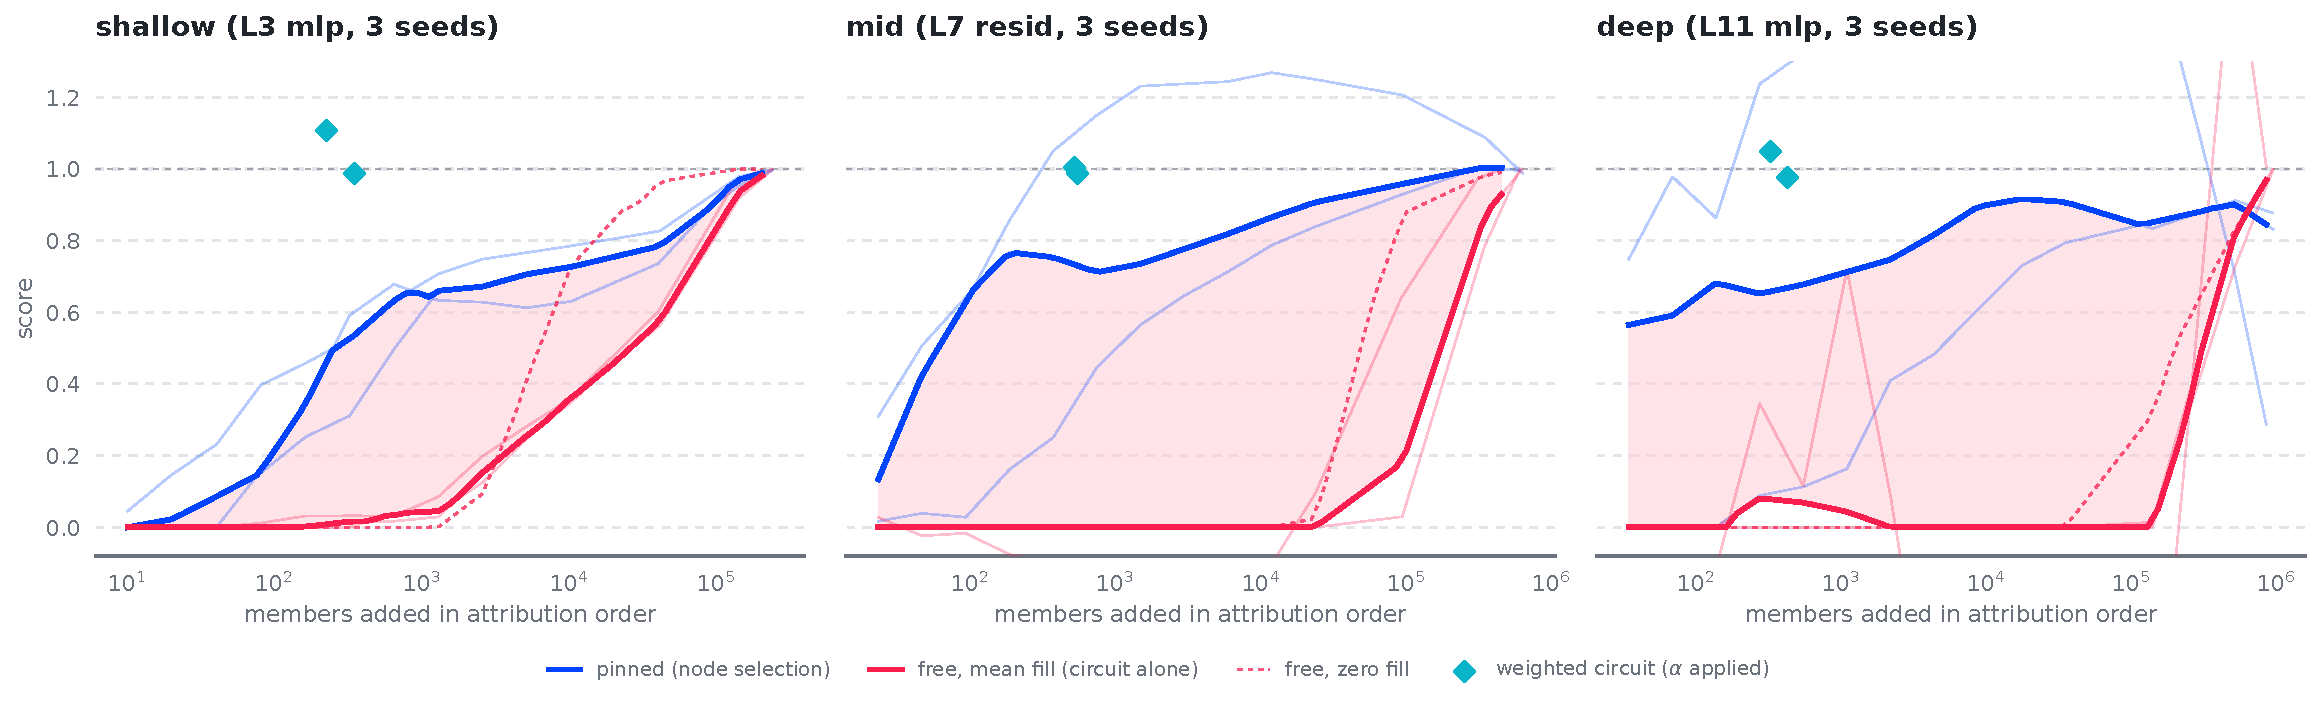
\includegraphics[width=\linewidth]{control-vs-faithfulness.pdf}
\caption{Control is sparse; faithfulness is collective.
Cumulative score against members added in attribution order (one seed per depth band; position-aware path attribution, percentile selection): pinned faithfulness (node selection) rises steeply and plateaus near 1 by $10^{2}$--$10^{3}$ members, while free faithfulness (the circuit alone) sits at zero until $10^{4}$--$10^{5}$ members and rises with a long tail of individually negligible ones --- under the mean fill (solid) and the zero fill (dashed), each free variant naming its semantics.
The shaded pinned--free gap widens with seed depth.}
\label{fig:drivers-closure}
\end{figure}

\subsection{Weighted Circuits: Amplitudes Index the Faithfulness Cost}
\label{sec:weighted}
% TRI-AMP PASS 2026-08-07. Data: dev-notes/data/floor-isolation-2026-08-05
% R14-R21 (amp_rescore, amp_null, amp_cfsup, amp_stepsweep, amp_fastlam,
% amp_pnfloor). VINTAGE: 3-4 residual-stream seeds per depth (layers 2 and 9),
% 2-3 null draws per seed — a depth-stratified n>=16 panel, >=10 null draws,
% and attention/MLP seeds are owed before these numbers are final.

How much of the faithfulness cost is irreplaceable membership, and how much is redundancy that a re-weighted survivor could cover?
The free-amplitude mask (\cref{sec:ablmask}) asks the model directly, and the answer is most of it: on the calibration seeds, weighted circuits of $99$--$229$ latents at layer 2 and $242$--$653$ at layer 9 hold both zero-fill and mean-fill faithfulness within band ($0.90$--$1.13$), where gate-only memberships under the same acceptance need $5{,}000$--$18{,}000$ latents at depth --- a $4$--$31\times$ collapse from amplitude freedom alone.
The central finding is thereby \emph{indexed}, not overturned: at natural amplitudes, faithfulness costs orders of magnitude more than interventional control; grant each member a learned scalar and one compact circuit passes both criteria.
The collective tail of \cref{sec:drivers-closure} is largely amplitude-compensable redundancy --- many latents each carrying a small share of a signal that fewer, rescaled members can carry alone --- which is exactly what the collective-faithfulness picture predicts.

\paragraph{The null that makes the claim safe.}
Free coefficients invite the objection that \emph{any} spanning set could be fitted to reconstruct the seed.
It cannot: random same-size sets drawn from the live latent pool, given the identical amplitude-fitting budget on their own members, fail on every draw at both depths --- zero-fill faithfulness $3.6$--$21$ at layer 2 and $10^{3}$--$2 \times 10^{4}$ at layer 9 against the discovered circuits' ${\sim}1$, with mean-fill faithfulness exactly $0.0$ on every random draw.
Weighted-circuit faithfulness is a property of the selected membership, not of the fitting capacity of its coefficients.

\paragraph{The amplitudes carry causal weight.}
Necessity is unchanged by re-weighting (suppression $0.99$--$1.02$ on all six seeds), and at layer 2 the amplitudes themselves are load-bearing on a task they were never fitted to: injecting members at their clean values drives the seed to only ${\sim}0.6$ on held-out negative contexts, while injecting them at $\alpha \times$ clean values drives it to $0.90$--$1.25$.
At layer 9 the picture is heterogeneous --- two seeds drive at bare clean values already (with the amplitudes overshooting, $1.38$--$1.50$), and one reconstructs perfectly yet barely drives ($0.25$) --- and that heterogeneity turns out to be an artifact of the training budget, measured next.

\paragraph{The budget is part of the method.}
Sweeping the training budget shows reconstruction faithfulness converges by $100$ steps; everything after buys sparsity, and it pays for it in drive calibration, which decays monotonically with training in five of six seeds --- the non-driving layer-9 circuit above \emph{drives} ($0.88$) when discovered at a quarter of the budget, its drive-carrying members progressively pruned thereafter ($0.88 \rightarrow 0.57 \rightarrow 0.25$).
Sparsity bought by budget and sparsity bought by price are also \emph{different circuits}: at matched size the two prunings share only about half their members --- a fifth underdetermination probe (\cref{sec:underdetermination}).
Two further semantics results close the loop.
Amplitude-only training on a frozen membership does not fix the drive overshoot but does inflate amplitudes monotonically --- the objective simply does not constrain the drive axis --- and removing the zero-ablation term from training explodes zero-fill faithfulness to $36$--$1{,}681$ at depth while the trained fill stays in band: the sharpest of six demonstrations that a method wins exactly the metric whose semantics it trains, now at the level of coefficients rather than membership.
The training schedule therefore belongs in the method statement, chosen per claim: the full budget for the most compact circuit, a quarter of it (at a raised price) when drive fidelity is the point.

\subsection{Method Comparison at Matched Size}
\label{sec:method-comparison}
% STEP 5 DONE as a FRAME (2026-07-30) — GATED on the definitive current-recipe
% matrix + the lambda re-anchor; the numbers below are earlier-recipe vintage
% and are phrased as directional. Replace with the matrix table when it lands.

Three discovery families compete for the same object --- attribution-threshold arms (\cref{sec:modes,sec:membership}), the learned mask (\cref{sec:ablmask}), and full-trajectory restoration --- and a complete head-to-head at matched size on the final recipe is queued, so magnitudes here are directional.
Three results structure the comparison.
First, restoration must complete its trajectory: with the round budget raised to the seed's upstream site count, deep-seed free faithfulness moves from $0.16$ to ${\sim}0.98$ --- the strongest method on that criterion at every depth we measured, at ${\sim}4\times$ the cost; the earlier deep failures were a rounds ceiling, not a second wall (\cref{app:mode-studies}).
Second, the learned mask posts the tightest zero-ablation faithfulness we have measured ($0.002$--$0.10$ from unity), and the dual floor beats its single-floor ablations at matched size on every seed of its comparison.
Third --- and the reason no single number can rank methods --- the \emph{home-turf effect}: a method wins the metric whose semantics it trains, observed three separate ways (a zero-floor mask leads on \texttt{free0}; a negctx-floor mask leads on \texttt{freeN\_topk} while its \texttt{free0} collapses; annealing sharpens the hard-set anchor while conceding on fills).
Rankings are therefore a matrix of method against semantics at matched size --- a single column mostly reveals which semantics did the scoring.

\subsection{Method and Negative Mode}
% STEP 5: v1 subsection, RETAINED (random-beats-close is a keeper finding;
% B7 ties it to the negctx-precedent literature; preact-filter hypothesis from
% B6m may add a sentence once Sweep 1 lands).

\begin{figure}
\centering
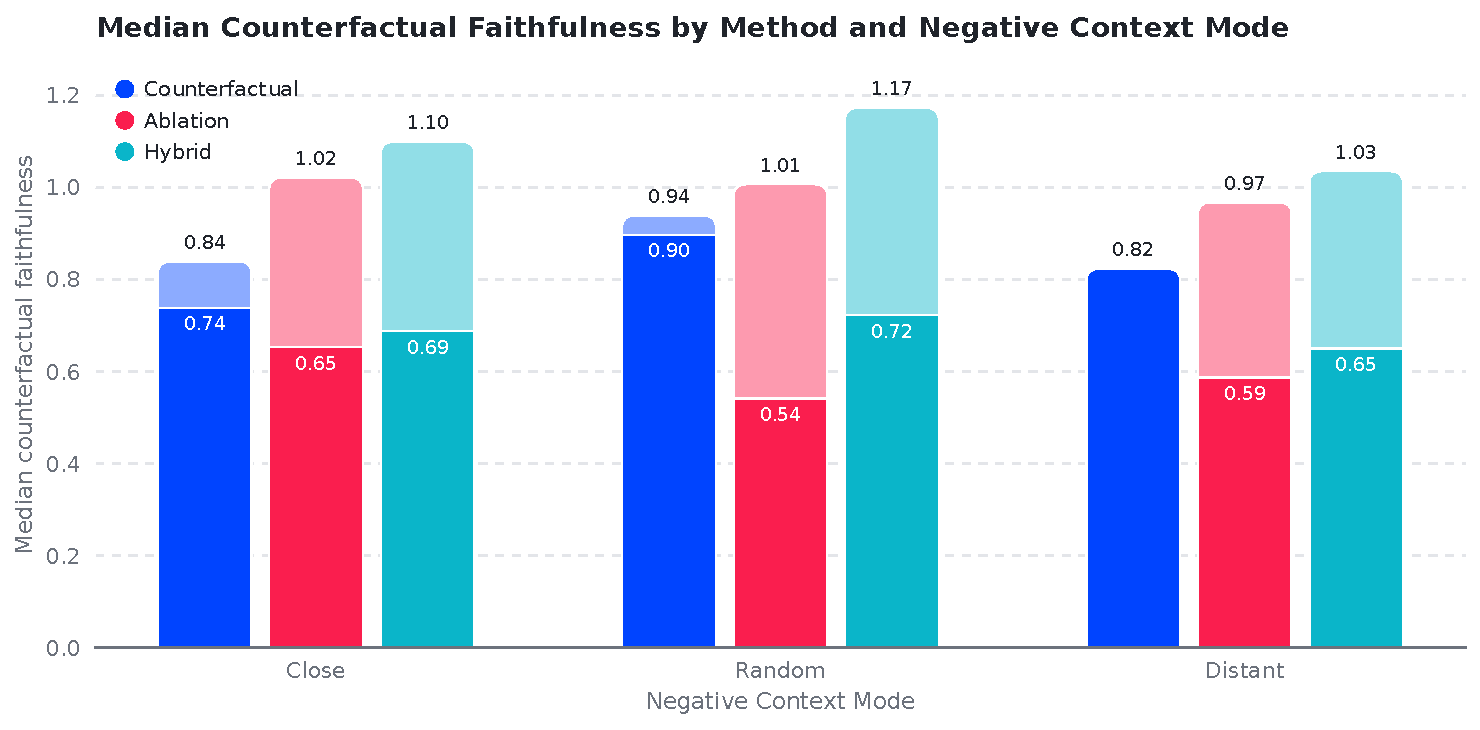
\includegraphics[width=0.85\linewidth]{median-cf-faithfulness.pdf}
\caption{Median counterfactual faithfulness by discovery method and negative mode.
Solid segments are medians over each method--mode group's accepted circuits; light segments extend to the median of the group's 44 highest-faithfulness circuits, 44 being the smallest accepted count among the nine groups, for an equal-population comparison.
Negative modes are \emph{close} (hard negatives retrieved by nearest-neighbour similarity), \emph{random} (uniformly sampled sequences), and \emph{distant} (sequences maximally dissimilar to the positive contexts).}
\label{fig:median-cf-faithfulness}
\end{figure}

Counterfactual gradient achieves the highest median faithfulness across all three negative modes, peaking at approximately 0.90 with random negatives.
Its advantage over ablation gradient is largest in the random condition (0.36), intermediate in the distant condition (0.24), and smallest in the close condition (approximately 0.09).
This ordering makes mechanistic sense: counterfactual gradient is explicitly optimised for the faithfulness criterion, while ablation gradient targets suppression and achieves faithfulness as a by-product.

The effect of negative mode is itself a finding.
One might expect close negatives --- semantically similar to the positive contexts but lacking the seed's activation --- to produce the sharpest contrastive signal.
In practice the reverse holds for counterfactual gradient: random negatives outperform close negatives by approximately 0.16 median faithfulness points.
The most likely explanation is that close negatives, being near the positive distribution, partially activate the seed's mechanism, providing a noisy gradient signal --- exactly the unverified-negatives gap of \cref{sec:evidence} --- while random negatives, where the seed is more completely absent, produce a cleaner gap and a more reliable attribution.
Semantic closeness and clean causal contrast, in other words, are not the same property, and negative-context construction should be treated as an experimental variable rather than a solved preprocessing step; verified-inactivity filtering and distribution-matched negatives are the natural next steps.

\subsection{Membership Is Underdetermined; Function Is Not}
\label{sec:underdetermination}
% STEP 5 DONE (2026-07-30; B6l + B6p — the solidest numbers in the section,
% bit-determinism established before any probe was run).

The learned-mask pipeline is bit-deterministic at fixed settings --- two identical runs agree to six decimal places with \emph{zero} membership flips --- so nothing below is run-to-run noise, and tiny perturbations become controlled experiments on the objective itself.
Five probes give the same verdict.
\begin{itemize}
\item \textbf{Precision.} A float32 and a bfloat16 run differ only in rounding, yet share a membership Jaccard of $0.835$ at layer 8 ($16.5\%$ of members exchanged; $0.803$ at layer 10) while \texttt{free0} is a wash ($1.058$ vs $1.060$) and size agrees within $2\%$ --- a rounding-scale perturbation lands a different, equally good member set.
\item \textbf{Sparsity path.} Raising $\lambda$ swaps members rather than nesting them: containment between consecutive steps runs $0.49$--$0.80$, and the cleanest cell changes size by $4.6\%$ and held-out loss by $4.5\%$ while replacing $50.8\%$ of the membership.
\item \textbf{Time.} No gate ever freezes, under any schedule we tested; a half-training snapshot is $57$--$72\%$ oversized and the second half of training removes $36$--$42\%$ of its members, so the stopping step is one more sampling axis.
\item \textbf{Threshold.} $8$--$25\%$ of members sit within $0.05$ of the decision cut and are load-bearing: cutting a trained mask down to a target size is strictly worse than training the price to that size ($0.126$ vs ${\sim}0.7$ on \texttt{free0} at matched size).
\item \textbf{Budget.} At matched size, a short-budget high-price run and a long-budget low-price run share only $0.40$--$0.53$ of their members by Jaccard --- and the two prunings differ functionally, with the long budget preferentially deleting drive-carrying members (\cref{sec:weighted}).
\end{itemize}
The organising claim: \textbf{aggregates are smooth; membership is not.}
Size falls monotonically with the sparsity price and faithfulness is stable under all five perturbations, but \emph{which} latents make the cut is identifiable only to the ${\sim}16$--$20\%$ level from 64 probe sequences: a discovered membership is one sample from the family $\Phi_{\varepsilon}$ of \cref{sec:problem}, and these probes measure the family's breadth.
We therefore report memberships as size-calibrated families, phrase per-latent claims accordingly, and let set-level and functional claims --- which the perturbations leave untouched --- carry the paper's conclusions.

\subsection{The Behaviour-Endpoint Boundary}
\label{sec:sfc-boundary}
% STEP 5 DONE (2026-07-30; B6g/B6h, symmetry framing per B6j). Re-run with the
% definitive matrix batch before final numbers are quoted.

To measure where the latent endpoint parts from the behavioural one, we replicated sparse feature circuits as a first-class method on our own model and SAE bank --- the same evidence base and the same seeds --- so the comparison is method against method, not architecture against architecture.
The replication follows the published specification for this setting: single-input zero-ablation indirect effects, with position-aggregated nodes as prescribed for non-templatic data~\citep{marks2025sparse}.

Each approach wins its own endpoint, exactly.
Behaviour-endpoint circuits, even at their most permissive threshold, score $\phicf = \phisup = 0.000$ on every seed: nodes selected to explain a logit contain nothing that controls whether a chosen internal latent fires.
Symmetrically, our circuits score near zero on logit faithfulness: they populate the seed's causal prefix, not the output pathway.
We read this as symmetry, not failure in either direction --- a scope result: ``which features support this output?'' and ``what makes this feature fire?'' are different questions whose answers share essentially no nodes, and because both directions share the same attribution estimator (\cref{sec:modes}), the separation isolates the endpoint and the membership rule rather than estimator quality.
One caveat bounds the reading: the behaviour-endpoint arm ran at its ceiling threshold without a held-out split, so this is a scope result, not a comparative one --- a threshold sweep is owed before any ranking claim.

\subsection{Dependencies Are Not Recoverable from Co-activation}
\label{sec:coact-results}
% STEP 5: v1 subsection, RETAINED (correlational baselines fail intervention
% gates outright — still a load-bearing argument for causal discovery).

If the discovered dependencies were merely co-occurrence in disguise, the co-activation graph would predict them.
It does not.
In a full-scale run of the gradient methods producing 7{,}525 accepted circuits, the mean overlap between a circuit's discovered nodes and its seed's top co-activation neighbourhood was approximately 3.6\%, the mean pairwise co-activation density among discovered nodes was approximately 0.26\%, and neither quantity correlated with counterfactual faithfulness (Pearson $r = 0.02$; distributions in \cref{fig:coact-overlap}).
Latent co-activation profiles across the bank are themselves nearly orthogonal --- the first two principal components explain roughly 3\% of variance --- so local co-occurrence structure carries little of the information that gradient-based contrast discovers.
Causally validated dependency neighbourhoods, in short, are not local co-activation neighbourhoods.

The converse test is to let co-activation structure propose circuits directly.
Under the same 128-seed protocol, evidence base, and seed-intervention gates, two correlational baselines from the method catalogue (\cref{app:methods}) --- sparse co-activation expansion, which follows the strongest co-activation edges outward from the seed, and differential activation, which ranks latents by their positive-versus-negative activation contrast --- produced no accepted circuits at all, while ablation gradient accepted circuits for 121 of the same 128 seeds (\cref{tab:coact-methods}).
Correlational proposals do not merely score lower; they fail the intervention gates outright.

The same run reveals a pattern that warrants caution: a small set of non-seed latents (233 of roughly 800{,}000 unique) recurs in at least 15\% of circuits, overwhelmingly as early-layer counterfactual inhibitors.
Whether these are genuinely shared regulatory machinery or an artefact of the discovery objective --- any generic suppressive direction can help close the pre-activation gap --- requires per-latent null tests that we leave to future work.

\section{Discussion}
\label{sec:discussion}
% STEP 6 DONE (2026-07-30): thesis-led reorganisation; Reframes 1–3 in the
% softened build-on voice; v1 keeper paragraphs retained below.

\paragraph{Circuit size is a measurement, not a knob.}
The faithful memberships of \cref{sec:drivers-closure} are large --- tens of thousands of latents for deep seeds --- and the standard reflex is to read that as a defect to be minimised.
The decomposition says otherwise.
Two success criteria were colliding under the single word ``circuit'': \emph{interventional control}, which a compact circuit passes, available from the same discovery pass; and \emph{faithfulness}, whose cost is a measured quantity.
Because a compact controlling circuit can always be exhibited, the faithfulness cost is free to be honest: it reports how much of the stream the latent's computation actually reads.
And faithfulness is a \emph{collective} property: every member is individually removable at the measurement floor, yet bulk removal by the members' own ranking craters the seed --- so any selection rule that thresholds individual contributions will undercount it systematically, however its threshold is tuned.
A latent's activation, reached through an additive residual stream, is a dense function of many small contributions, and no sparse threshold captures a dense function.
The weighted-circuit results sharpen the thesis rather than soften it: the cost is a measurement \emph{at stated amplitude semantics} --- most of the collective tail is redundancy a rescaled survivor can carry (\cref{sec:weighted}) --- so a circuit's size is meaningful only alongside the amplitude convention it was measured under.

\paragraph{Evaluation semantics are part of the method.}
\citet{miller2024transformer} showed that faithfulness is not robust to the choice of ablation; our measurements push the same point one level down: the semantics reach the \emph{training objective} itself.
The intervention pair already shows it at the acceptance gate --- $\phicf$ and $\phisup$ operationalise different claims, sufficiency to impose and necessity to sustain, and each method's accepted circuits look best on the metric it gates on --- and the home-turf effect shows it in training: a method wins the metric whose semantics it trains, three separate ways (\cref{sec:method-comparison}).
Two consequences follow: rankings are a matrix of method against semantics at matched size, and semantics can be \emph{designed for} rather than merely suffered --- the multi-floor loss trains one membership under up to three ablations jointly.
The strongest quantitative form of the point is about membership itself: memberships trained under different floors share fewer latents than memberships trained for different objectives (Jaccard $0.13$ against $0.54$ at matched size) --- the counterfactual matters more than the target --- and for weighted circuits the semantics reach the coefficients too, where an untrained axis is not merely unmeasured but miscalibrated by orders of magnitude (\cref{sec:weighted}).
Discovery, training, and evaluation semantics belong in the method statement, not in a footnote.

\paragraph{Report memberships as families.}
The underdetermination results (\cref{sec:underdetermination}) change what a responsible membership claim looks like.
Set-level and functional claims --- size, faithfulness, the cost findings --- are stable under every perturbation we applied.
Per-latent claims (``latent $g$ belongs to seed $f$'s circuit'') are not, at the ${\sim}16$--$20\%$ level, from 64 probe sequences: the objective admits a family of near-equivalent optima, and a single run samples one member.
Claims of the first kind carry this paper; claims of the second kind require survival across perturbations --- precision, sparsity path, stopping step --- before they are asserted, and the same redundancy that frustrates them is itself a finding: many latents each doing a small share of the same job is exactly what the collective-faithfulness picture predicts.

\paragraph{Generality has a price, and we pay it in the open.}
Position handling in prior circuit work offers three strategies, each right for its setting: position-indexed nodes where a template fixes roles, per-instance graphs built one prompt at a time, and schema-based alignment of variable-length examples (\cref{sec:membership} cites each).
The membership set extends this line to the setting none of them targets --- one reusable circuit over arbitrary non-templatic text with a sharp latent endpoint --- and at that endpoint, compactness and faithfulness trade off directly.
We therefore report the full faithfulness-versus-size curve rather than a single operating point, with the compact controlling circuit available whenever a small interpretable object is wanted.

\paragraph{From neighbourhoods and memberships to chains.}
The co-activation results close a loop in the premise: if latent dependencies were recoverable from co-occurrence, the latent-endpoint programme could be served by cheap statistics --- and they are not.
The discovered objects remain seed-indexed: signed one-hop dependencies, and a membership that reproduces the seed alone.
Neither is yet a multi-hop pathway.
Because every object is indexed by its seed, composition is available in principle --- splice the circuit that explains an upstream latent into the circuits that use it, then re-validate by intervening at the earliest nodes and measuring propagation through intermediates --- and the faithfulness results set its boundary condition: a composed chain inherits the faithful memberships of its links, so composition must manage membership, not merely concatenate stars.
That composition-with-validation step, rather than more discovery methods, is the path from dependency neighbourhoods to genuine circuits.

\section{Limitations}
\label{sec:limitations}
% STEP 6 DONE (2026-07-30). The "Panel scale and open runs" item names the two
% open gates — reword or remove it if they close before submission.

\textbf{The SAE basis is not ground truth.}
Latents are more interpretable than neurons on average, but many resist clean characterisation, and circuits built from ambiguous latents inherit that ambiguity; our metrics measure intervention effects, not interpretability.

\textbf{The objective is a surrogate, and can have artefacts.}
A high pre-activation does not guarantee a Top-K slot, so attribution optimises a continuous surrogate of a discrete event; annealed binarisation closes the training half of that gap, but the surrogate remains in every attribution mode, and evaluation closes the loop only at the point of intervention.
Relatedly, high-commonality early-layer inhibitors could be generic suppressive directions rather than mechanism-specific regulation --- any suppressor helps close the pre-activation gap --- and per-latent null tests are needed.

\textbf{Multi-hop structure is composed, not discovered.}
The position-collapsed faithfulness failure that once sat here as an untested caveat is now a diagnosed mechanism with a measured fix (\cref{sec:membership,sec:drivers-closure}); what remains true is that discovered graphs are one-hop neighbourhoods and memberships are sufficiency sets, not wired pathways, and unvalidated compositions should not be over-interpreted.

\textbf{Negative contexts are not verified counterfactuals.}
Retrieval excludes stored positives but does not verify seed inactivity, and pooled final-layer representations are an imperfect proxy for semantic similarity; a pre-activation filter for near-miss negatives is implemented but not yet swept, so random negatives double as the operational mitigation (\cref{sec:results}).

\textbf{Per-latent membership is not identifiable from a single run.}
Perturbations at the level of float rounding exchange ${\sim}16$--$20\%$ of members at unchanged quality (\cref{sec:underdetermination}); we phrase claims at the set and function level accordingly, and per-latent claims require survival across perturbations, which single-run studies --- including ours, where not otherwise stated --- do not establish.

\textbf{Protocol debts.}
No strict held-out split is enforced (ablation gradient attributes and evaluates on the same probe set, and pruning optimises the acceptance metric), so reported scores are in-distribution intervention performance; the control/faithfulness magnitudes come from panels of three to sixteen seeds, pending the depth-stratified full-scale run and the final cross-method matrix; and the size-calibration exponent is recipe-bound, re-fit whenever the training dynamics change.
The weighted-circuit results are the youngest and thinnest panel: three to four residual-stream seeds per depth at two layers, two to three amplitude-fitted null draws per seed against a drive null with a measured heavy tail, and probes drawn from each seed's own firing distribution --- a depth-stratified panel, ten-plus null draws, attention and MLP seeds, and held-out contexts are owed before those numbers are final.

\textbf{Generality.}
TuringLLM's synthetic corpus is an asset for epistemic control but a limit on generality, and intervention-based evaluation itself places the model in execution contexts it was not trained in.
Replication on a public model with public SAEs is a priority.

\section{Conclusion}
% STEP 6 DONE (2026-07-30): matched to the six-contribution list.

This paper reframed circuit discovery around an internal endpoint --- not \emph{which features caused this output} but \emph{what makes this feature fire} --- and followed the reframing to its two criteria: signed one-hop dependencies validated by intervention, and the membership a latent needs before the circuit alone reproduces it.
The machinery is matched to the endpoint: pre-activation attribution and objectives that survive seed silence and Top-K censoring, learned-mask discovery trained under up to three ablation semantics at once with learned per-member amplitudes, and an evaluation family that separates node selection from faithfulness proper and names its semantics on every score.
The empirical lessons run in one direction: interventional control is concentrated while faithfulness is collective, position-local, and depth-scaled at natural amplitudes --- and amplitude freedom collapses its cost by orders of magnitude, so circuit size is meaningful only with its amplitude convention; each method wins the metric whose semantics it trains, so rankings are a matrix, not a column; membership is underdetermined while function is stable, so circuits are families, not sets; negative-context construction materially changes what is discovered; none of it is recoverable from co-activation statistics; and none of it is reachable from behavioural endpoints.

The honest status of the output is \emph{causally validated local dependencies, and measured faithfulness costs, for SAE latents} --- not yet a dependency graph over the model's internal ontology.
Reaching the stronger claim has a concrete path: depth-stratified scale-up of the membership results, held-out intervention protocols with matched null controls, composition of seed-indexed circuits into chains with propagation tests, and replication beyond a single controlled model.
The infrastructure and evaluation regime built here are designed to make each of those steps a measurement rather than an argument.

\section*{Reproducibility}
The full system --- pipeline stages, evidence stores, the gradient discovery methods of \cref{sec:method}, the seed-intervention evaluation, and the analysis code that produces every figure and table in this paper --- is available at \href{https://github.com/DanielJamesDavies/turing-explorer-circuit-discovery}{\nolinkurl{github.com/DanielJamesDavies/turing-explorer-circuit-discovery}}.
TuringLLM, its synthetic training corpus, and the trained SAE bank are described in \cref{app:corpus}; the grid experiment of \cref{sec:results} is reproducible from the released configuration, and each analysis reads only the run artifacts written by the pipeline stages.

\bibliographystyle{plainnat}
\bibliography{references}

\appendix
\crefalias{section}{appendix}
\crefalias{subsection}{appendix}
\crefalias{subsubsection}{appendix}

\section{Corpus and Model Details}
\label{app:corpus}

\subsection{A Corpus Built by Design}

The synthetic corpus was constructed in two stages.
The first produced a relatively small but high-quality foundation: Phi-3 Mini~\citep{abdin2024phi3}, a 3.8B-parameter language model available under a permissive licence, generated instructional and educational text spanning 18 broad subject areas (Physics, Mathematics, Computer Science, Chemistry, Biology, Philosophy, English, Creative Writing, Languages, Art, Music, Engineering, Economics, Business, Geography, History, Culinary Arts, and Communication), recursively generating topics and sub-topics and producing structured documents of headings and text.

The second stage addressed scale.
A fine-tuned T5-based paraphrase model~\citep{vorobev2023paraphraser, raffel2020exploring} expanded the corpus by generating 11 paraphrased variants of each source document, motivated by knowledge distillation results~\citep{ba2014deep, hinton2015distilling} suggesting that varied outputs of a stronger teacher can be advantageous over raw data alone.
The final corpus totals approximately 2 billion tokens.

Two tokenized datasets were derived using the Phi-3 Mini tokenizer.
The language-modelling training set combines original and augmented texts shuffled into epochs, concluding with a second pass over only the high-quality originals to consolidate representations around the cleaner signal.
The interpretability dataset consists of 64-token chunks shuffled into 4,096 shards, allowing the pipeline to process one shard at a time with a bounded memory footprint.

\subsection{Architecture and Training}

\begin{table}
\centering
\begin{tabular}{ll}
\toprule
\textbf{Attribute}         & \textbf{Value}  \\
\midrule
Parameters                 & 254M            \\
Layers                     & 12              \\
Residual stream dimension  & 1,024           \\
Attention heads            & 16              \\
MLP hidden dimension       & 4,096           \\
Context length             & 1,024 tokens    \\
Vocabulary size            & 50,304 tokens   \\
MLP activation             & SwiGLU          \\
Normalisation              & RMSNorm         \\
Tokenizer                  & Phi-3 Mini      \\
\bottomrule
\end{tabular}
\caption{TuringLLM-1.0-254M architecture summary.}
\label{tab:turinglm}
\end{table}

TuringLLM follows the residual-stream design of the GPT family~\citep{radford2019language} with two deliberate departures: SwiGLU~\citep{shazeer2020glu, ramachandran2017searching} replaces the ReLU MLP, following the motivation of the Llama family~\citep{touvron2023llama}, and RMSNorm~\citep{zhang2019root} replaces layer normalisation.
\Cref{fig:architecture} sketches the architecture.
Training reached a minimum cross-entropy of approximately 1.62 (train) and 1.80 (validation); the same infrastructure applied to GPT-2 (124M) reaches approximately 3.29~\citep{karpathy2024nanogpt}, reflecting the tighter distribution of the synthetic corpus.
The loss curve (\cref{fig:loss-curve}) drops sharply in its final phase, corresponding to the second pass over Phi-3 Mini originals.

\begin{figure}
\centering
\scalebox{0.85}{%
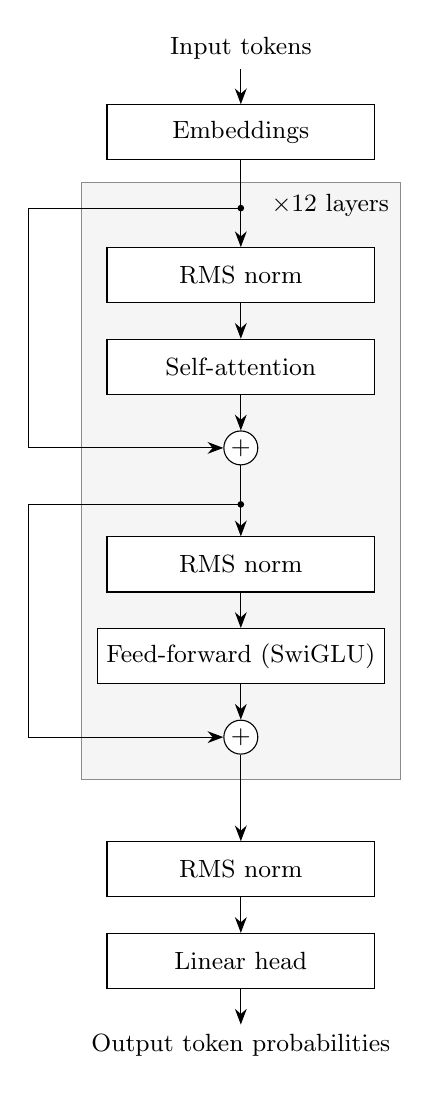
\begin{tikzpicture}[
  font=\small,
  box/.style={draw, rectangle, minimum width=3.4cm, minimum height=0.7cm, align=center, fill=white},
  sum/.style={draw, circle, inner sep=1pt, fill=white},
  arrow/.style={-{Stealth[length=2mm]}},
  node distance=0.45cm
]
\node (input) {Input tokens};
\node[box, below=of input] (emb) {Embeddings};
\node[box, below=1.1cm of emb] (norm1) {RMS norm};
\node[box, below=of norm1] (attn) {Self-attention};
\node[sum, below=of attn] (add1) {$+$};
\node[box, below=0.9cm of add1] (norm2) {RMS norm};
\node[box, below=of norm2] (mlp) {Feed-forward (SwiGLU)};
\node[sum, below=of mlp] (add2) {$+$};
\node[box, below=1.1cm of add2] (fnorm) {RMS norm};
\node[box, below=of fnorm] (lin) {Linear head};
\node[below=of lin] (out) {Output token probabilities};

\coordinate (skip1) at ($(emb.south)!0.55!(norm1.north)$);
\coordinate (skip2) at ($(add1.south)!0.55!(norm2.north)$);

\draw[arrow] (input) -- (emb);
\draw[arrow] (emb) -- (norm1);
\draw[arrow] (norm1) -- (attn);
\draw[arrow] (attn) -- (add1);
\draw[arrow] (add1) -- (norm2);
\draw[arrow] (norm2) -- (mlp);
\draw[arrow] (mlp) -- (add2);
\draw[arrow] (add2) -- (fnorm);
\draw[arrow] (fnorm) -- (lin);
\draw[arrow] (lin) -- (out);

\fill (skip1) circle (1.2pt);
\draw[arrow] (skip1) -- ++(-2.7,0) |- (add1.west);
\fill (skip2) circle (1.2pt);
\draw[arrow] (skip2) -- ++(-2.7,0) |- (add2.west);

\coordinate (boxtop) at ($(norm1.north)+(0,0.5)$);
\begin{scope}[on background layer]
\node[draw=black!45, fill=black!4, inner sep=9pt, fit=(boxtop)(norm1)(attn)(add2)(skip2)] (layerbox) {};
\end{scope}
\node[anchor=north east, inner sep=4pt] at (layerbox.north east) {$\times 12$ layers};
\end{tikzpicture}%
}
\caption{TuringLLM-1.0-254M architecture: a 12-layer pre-norm decoder-only transformer with \mbox{RMSNorm} and a SwiGLU feed-forward block.
The circuit-discovery pipeline attaches SAEs at three sites per layer: attention output, MLP output, and the residual stream.}
\label{fig:architecture}
\end{figure}

\begin{figure}
\centering
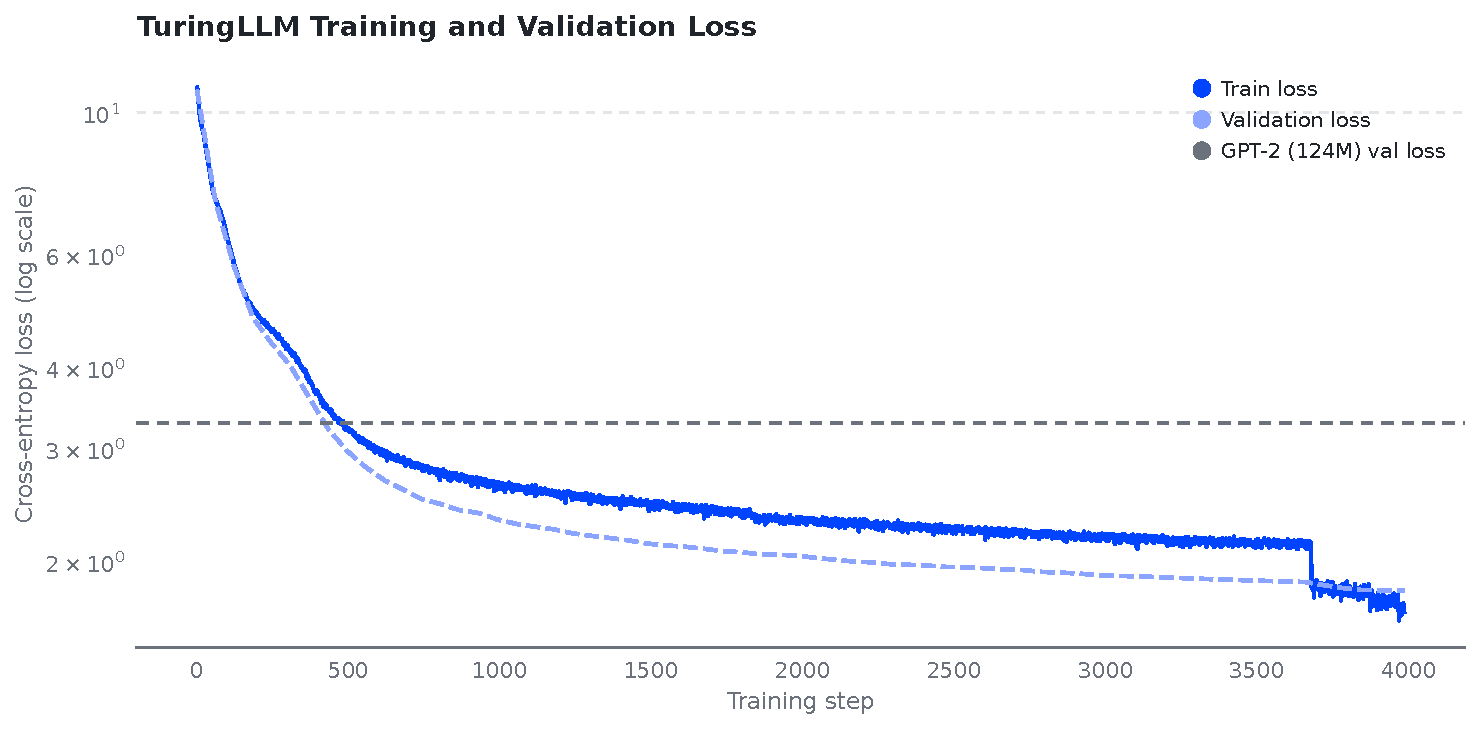
\includegraphics[width=0.9\linewidth]{loss-curve.pdf}
\caption{TuringLLM training and validation cross-entropy over the 3{,}985-step run (log scale).
The dashed reference marks the validation loss reached by the same training infrastructure applied to GPT-2 (124M); the drop near step 3{,}700 corresponds to the final pass over only the high-quality Phi-3 Mini originals.}
\label{fig:loss-curve}
\end{figure}

\subsection{Fitness for Interpretability}

TuringLLM is not designed to win benchmarks; it is designed to be a controlled subject.
Standard held-out benchmarks fit poorly for a base model trained on synthetic educational text, so fitness was evaluated qualitatively and through structured internal tests: Phi-3 Mini composed topic-specific opening sentences and scored TuringLLM's completions on English quality and topic adherence, yielding average grades of approximately B and A respectively across the 18 subject areas.
This level of competence supports the working hypothesis that the model contains structured internal representations worth studying; a model merely interpolating noise would not produce consistently topical completions.
Representative completions are shown in \cref{fig:completions}.

\subsection{Sparse Autoencoder Quality}
\label{app:sae-quality}

\Cref{fig:sae-quality} reports three standard quality metrics for the 36-SAE bank, per site.
\emph{Explained variance}, $1 - \operatorname{Var}(x - \hat{x}) / \operatorname{Var}(x)$, measures reconstruction fidelity.
\emph{Alive latents} is the fraction of each dictionary's 40,960 latents that fired at least once during the full collection pass over the interpretability corpus.
\emph{Loss recovered} splices each SAE's reconstruction into the model at its site and reports the recovered share of the cross-entropy gap between the original model and zero-ablating that site~\citep{marks2025sparse}, measured over 12{,}288 held-out corpus tokens.
Because the SAEs are Top-K with $K = 128$, sparsity is fixed by construction and the usual $L_0$--fidelity trade-off curve is a single point per SAE.

Three observations matter for interpreting the paper's results.
First, reconstruction fidelity is healthy across the bank: attention SAEs explain 0.93--0.99 of variance, residual SAEs decline smoothly with depth to 0.85, and MLP SAEs bottom out at 0.77 in layer 9.
Second, the layer-1 attention SAE has a dead-latent crater --- only 37\% of its latents ever fire (84\% at layer 2, at least 93\% everywhere else).
Third, loss recovered exposes a functional gap that explained variance misses: the layer-11 attention SAE recovers only 58\% of the cross-entropy gap despite explaining 0.96 of variance, indicating that the unexplained residual at the final attention site is disproportionately important to the logits.

These measurements sharpen the attention-seed result of \cref{app:extra-results}: the near-zero faithfulness of attention-seeded circuits is unlikely to be a reconstruction-fidelity problem, since attention SAEs are the bank's best reconstructors; the dead-latent structure and the final-layer functional gap are the more plausible suspects.

\begin{figure}
\centering
% MISSING FIGURE (lost in the 2026-07-22 teardown; figures/ was untracked).
% Regenerate from the SAE-quality analysis — see rewrite-tracker.md.
\fbox{\parbox[c][2.2in][c]{0.95\linewidth}{\centering\texttt{MISSING FIGURE: sae-quality.pdf}\\ (to regenerate — see rewrite-tracker.md)}}
%\includegraphics[width=\linewidth]{sae-quality.pdf}
\caption{Quality of the 36-SAE bank by site.
Left: explained variance of each SAE's reconstruction.
Middle: fraction of latents that fired at least once over the full collection pass.
Right: percentage of the cross-entropy gap recovered when splicing each SAE's reconstruction into the model, relative to zero-ablating the site.}
\label{fig:sae-quality}
\end{figure}

\begin{figure}
\centering
\small
\begin{tabular}{@{}p{0.95\linewidth}@{}}
\toprule
``Physics utilizes the fundamental concepts of quantum mechanics to explain how electrons populate a sublevel within an atom, which is marked by energy levels. These levels define the overall potential energy and enable electrons to occupy specific energy levels or sublevels [\ldots]'' \\[0.6em]
``Artificial Intelligence (AI) has played a pivotal role in elevating personalization in human-robot interfaces, elevating the potential for truly personalized and responsive user experiences. The evolution towards AI extends its roots back to the 1960s with early rule-based [\ldots]'' \\[0.6em]
``Artificial Intelligence (AI) and Machine Learning (ML) technology have become indispensable in modern engineering. These technologies enable engineers to analyze vast datasets with unprecedented efficiency, leading to significant improvements in design processes, maintenance, and optimization.'' \\
\bottomrule
\end{tabular}
\caption{Representative TuringLLM completions (excerpts).
Continuations are topical and grammatical, supporting the use of the model as an interpretability subject; occasional repetitions and factual slips (e.g.\ conflated terminology) reflect its 254M-parameter scale and synthetic corpus.}
\label{fig:completions}
\end{figure}

\section{Infrastructure and System Design}
\label{app:infra}

\subsection{A Model Built for Intervention}

The model runs in two modes.
In inference mode it is a standard decoder-only language model.
In hooked mode it exposes intermediate activations at every layer and component type, accepts surgical replacements of individual sparse features, and reports how those replacements propagate.
Every claim in circuit discovery ultimately rests on an intervention; without fine-grained access to internals, discovery is correlation.

\subsection{Pipeline and Stores}

The runtime separates the expensive from the reusable.
Running TuringLLM and all 36 SAEs over the corpus is the most computationally intensive operation and happens once per experiment; every subsequent analysis --- graph construction, candidate selection, discovery, evaluation --- reads from the artifacts the collection passes leave behind.
Because all discovery methods share the same evidence base, differences in their outputs are attributable to the methods rather than to differences in data seen.
Each latent has a persistent record: activation statistics, top/mid/negative context reservoirs, sequence representations, co-activation partners, and eventually circuit membership.

\subsection{Instrumentation and Patching}

Between stored evidence and evaluation sits the instrumentation layer: it records sparse activations during forward passes, exposes intermediate states through hooks, computes attribution by propagating gradients through those states, and applies patching operations that replace, inject, or suppress specific latent values.
SAE reconstruction residuals are preserved as explicit anchors at every hooked site, so interventions modify latent codes without absorbing reconstruction error into the measurement.
The same framework supports faithfulness tests, sufficiency checks, minimality pruning, counterfactual activation, and seed suppression.

\subsection{Native Kernels}

The SAE encoding path uses a Triton radix-select kernel for Top-K selection, a fused linear-ReLU encoder path, cublasLt matrix multiplication, and per-component CUDA stream parallelism; latent statistics, context reservoirs, and co-activation reductions are handled by custom C++/CUDA extensions.
The breadth of the experimental programme is feasible because these inner loops are fast.

\section{Pseudocode for the Gradient Methods}
\label{app:pseudocode}

\Cref{alg:cfgrad,alg:abgrad,alg:hybrid} summarise the discovery procedures of \cref{sec:cfgrad} as implemented; \cref{alg:restoration,alg:ablmask} summarise restoration-mode attribution (\cref{sec:modes}) and learned-mask discovery (\cref{sec:ablmask}).
Thresholds ($\tau_{\mathrm{act}}$, $\tau_{\mathrm{inh}}$, $\tau_{\mathrm{sup}}$, $\tau_{\mathrm{cf}}$, $\tau_{\mathrm{prune}}$) and top-$K$ sizes are configuration constants shared across the grid; upstream latents additionally require a minimum corpus active count $n_{\min}$, which filters dead or near-dead latents.
All forward passes run with identity passthroughs injected at every SAE site (\cref{sec:cfgrad}), so gradients flow to upstream latent activations, and the seed-intervention scores $\phicf$ and $\phisup$ are computed exactly as in \cref{sec:eval}.
Hybrid fusion (\cref{alg:hybrid}) unions the two circuits by feature identity, $\mathcal{F}^{\mathrm{hyb}} = \mathcal{F}^{\mathrm{cf}} \cup \mathcal{F}^{\mathrm{ab}}$, each node keeping its per-source scores and role labels and each directed edge inheriting the higher attribution; optional leave-one-out pruning drops nodes with negligible effect on either acceptance metric, and acceptance requires the fused circuit to clear the counterfactual and/or suppression thresholds, with the conjunction set per experiment.

\begin{algorithm}
\caption{Counterfactual gradient discovery (one seed $f$)}
\label{alg:cfgrad}
\begin{algorithmic}[1]
\Require seed $f$; positive contexts $\posset$; negative mode $m \in \{\text{close}, \text{random}, \text{distant}\}$
\State $\negset \gets \textsc{ContrastContexts}(f, m)$ \Comment{stored negctx, random corpus sequences, or maximally dissimilar sequences}
\State $\mu_f^{+} \gets$ mean seed activation over $\posset$
\State $(\tau_{\mathrm{act}}, \tau_{\mathrm{inh}}) \gets (\tau_{\mathrm{act}}, \tau_{\mathrm{inh}}) \cdot \max(\mu_f^{+}, 0.1)$ \Comment{scale thresholds so focal seeds are not penalised}
\For{each contrast sequence $x \in \negset$}
    \State forward pass; capture pre-activation $\preact(x, t)$ at the seed's site
    \State $t^{*} \gets \arg\max_t \preact(x, t)$;\quad $\Lcf(x) \gets \bigl(\preact(x, t^{*}) - \mu_f^{+}\bigr)^{2}$
    \State backward pass: $s_g^{\mathrm{cf}}(x) \gets a_g(x, t_g) \cdot \partial \Lcf(x) / \partial a_g(x, t_g)$ for every upstream latent $g$
\EndFor
\State $\Scf \gets \frac{1}{|\negset|}\sum_{x} s_g^{\mathrm{cf}}(x)$ for every $g$
\State activators $\gets$ top-$K$ latents by $\Scf$ with $\Scf \geq \tau_{\mathrm{act}}$ and active count $\geq n_{\min}$
\State inhibitors $\gets$ top-$K$ latents by $-\Scf$ with $|\Scf| \geq \tau_{\mathrm{inh}}$ and active count $\geq n_{\min}$
\State $C \gets$ star circuit $\{g \to f\}$ over activators $\cup$ inhibitors, edge weights $\Scf$
\If{$\tau_{\mathrm{prune}} > 0$}
    \State leave-one-out prune nodes whose removal changes $\phicf$ by less than $\tau_{\mathrm{prune}}$
\EndIf
\State $(\phicf, \phisup) \gets$ seed-intervention evaluation of $C$ on $\posset$ and $\negset$
\State \Return $C$ if $\phicf \geq \tau_{\mathrm{cf}}$, otherwise reject
\end{algorithmic}
\end{algorithm}

\begin{algorithm}
\caption{Ablation gradient discovery (one seed $f$)}
\label{alg:abgrad}
\begin{algorithmic}[1]
\Require seed $f$; positive probes $\posset$
\For{each positive probe $(x, t) \in \posset$}
    \State forward pass; backward pass from the seed's sparse activation $a_f(x, t)$
    \State $s_g^{\mathrm{ab}}(x) \gets a_g(x, t_g) \cdot \partial a_f(x, t) / \partial a_g(x, t_g)$ for every upstream latent $g$
\EndFor
\State $\Sab \gets \frac{1}{|\posset|}\sum_{x} s_g^{\mathrm{ab}}(x)$ for every $g$
\State supports $\gets$ top-$K$ latents by $\Sab$ above threshold, active count $\geq n_{\min}$
\State $C \gets$ star circuit $\{g \to f\}$ over supports (role: ablation support), edge weights $\Sab$
\If{$\tau_{\mathrm{prune}} > 0$}
    \State leave-one-out prune nodes whose removal changes $\phisup$ by less than $\tau_{\mathrm{prune}}$
\EndIf
\State $(\phicf, \phisup) \gets$ seed-intervention evaluation of $C$
\State \Return $C$ if $\phisup \geq \tau_{\mathrm{sup}}$, otherwise reject
\end{algorithmic}
\end{algorithm}

\begin{algorithm}
\caption{Hybrid gradient discovery (one seed $f$)}
\label{alg:hybrid}
\begin{algorithmic}[1]
\Require seed $f$; acceptance mode $\in \{\phicf, \phisup, \text{both, either}\}$
\State $C_{\mathrm{cf}} \gets$ \cref{alg:cfgrad} on $f$;\quad $C_{\mathrm{ab}} \gets$ \cref{alg:abgrad} on $f$ \Comment{either may reject}
\If{both rejected} \State \Return reject \EndIf
\State $C \gets$ fuse returned circuits by feature identity: union of nodes, each retaining its per-source attribution scores and role labels; each directed edge keeps the higher attribution
\If{$\tau_{\mathrm{prune}} > 0$}
    \State leave-one-out prune nodes with negligible effect on either acceptance metric
\EndIf
\State $(\phicf, \phisup) \gets$ seed-intervention evaluation of the fused $C$
\State \Return $C$ if the acceptance mode's condition holds ($\phicf \geq \tau_{\mathrm{cf}}$ and/or $\phisup \geq \tau_{\mathrm{sup}}$), otherwise reject
\end{algorithmic}
\end{algorithm}

\begin{algorithm}
\caption{Restoration-mode attribution (one seed $f$; \texttt{ig\_restoration} substitutes per-round integrated-gradient scoring in line 4)}
\label{alg:restoration}
\begin{algorithmic}[1]
\Require seed $f$; positive probes $\posset$; round budget $R$ = number of upstream sites; per-round admission size $k_r$
\State $M \gets \varnothing$; ablate every upstream latent (floor state)
\For{round $r = 1, \ldots, R$}
    \State forward with members $M$ live (re-encoded from the modified stream) and non-members ablated; capture the seed pre-activation $\preact$
    \State score every non-member $g$ by gradient-times-activation at the \emph{current} partially restored stream \Comment{re-linearisation: later rounds see the consequences of earlier admissions}
    \State $M \gets M \cup \{\text{top-}k_r \text{ non-members by score}\}$
    \If{$\preact$ is within tolerance of its natural value} \textbf{break} \Comment{restoration certificate}
    \EndIf
\EndFor
\State $C \gets$ circuit over $M$ with per-round scores; seed-intervention and ablation-faithfulness evaluation as configured
\State \Return $C$
\end{algorithmic}
\end{algorithm}

\begin{algorithm}
\caption{Learned-mask discovery (one seed $f$; house configuration shown)}
\label{alg:ablmask}
\begin{algorithmic}[1]
\Require seed $f$; positive probes $\posset$ with anchor positions; negative contexts $\negset$; sparsity price $\lambda$ (calibrated, \cref{sec:ablmask}); $\gamma = 0.25$; steps $S = 400$
\State target $\gets$ natural pre-activation of $f$ at the probe anchors (no-grad forward);\quad $\nu \gets \operatorname{mean}(\text{target}^2)$
\State collect negative-context site means (the fill floor); initialise $\theta_s$ for every upstream site $s$
\For{step $= 1, \ldots, S$}
    \State $T \gets 0.05^{\,\text{step}/S}$; \quad gates $m_s \gets \sigma(\theta_s / T)$ \Comment{geometric anneal $1 \rightarrow 0.05$}
    \State $\mathcal{L}_{\mathrm{zero}} \gets$ MSE of masked pre-activation against target under the zero floor
    \State $\mathcal{L}_{\mathrm{negctx}} \gets$ the same under the negative-context fill floor \Comment{same $\theta$, both semantics}
    \State AdamW step on $\bigl(\mathcal{L}_{\mathrm{zero}} + \gamma\,\mathcal{L}_{\mathrm{negctx}}\bigr)/\nu + \lambda \sum_{s,i} \sigma(\theta_{s,i})$
\EndFor
\State membership $\gets \{\,i : m_i > \tfrac{1}{2}\,\}$; evaluate under \cref{sec:eval-abl}
\State \Return membership
\end{algorithmic}
\end{algorithm}

\FloatBarrier

\section{Additional Discovery Methods}
\label{app:methods}

The system implements a broader catalogue of discovery methods than the gradient trio evaluated in the main text; all share the seed interface, evidence base, and evaluation pipeline.

\paragraph{Graph expansion family.}
Sparse co-activation expansion follows the highest-weight co-activation edges outward from the seed through variable-depth breadth-first search, with variants constrained by component type (attention-only, MLP-only, residual-only, and pairwise combinations), treating unexpanded kinds as passthrough.
Hard-negative co-activation expansion adds contrastive pressure by penalising latents strongly active on the seed's negative contexts and validating candidate inhibitors with attribution.

\paragraph{Gradient-free baselines.}
Threshold-based co-activation selection includes any neighbour whose stored edge weight clears a fixed threshold; two-hop neighbourhood expansion grows a bounded structural neighbourhood with explicit branching factors.
These exist as reference points: an elaborate method that cannot outperform simple graph structure is not earning its complexity.

\paragraph{Output-rooted attribution methods.}
Logit attribution scores nodes and edges by activation-times-gradient against output logits.
An SFC-style method~\citep{marks2025sparse} computes integrated-gradient node scores against a patch baseline with typed edge attribution.
An SAE-adapted implementation of attribution graphs~\citep{ameisen2025circuit} enumerates all active latents, ranks features by logit influence, fills a direct-effects matrix by per-feature backward passes, propagates influence by Neumann series, and prunes by influence-mass fractions.

\paragraph{Contrastive statistical method.}
Differential activation ranks latents by mean activation difference between positive and hard-negative contexts, proposing activators and inhibitors that are then validated with gradient attribution on positive tokens.

\section{Context Stores, Selection Criteria, and Output-Level Metrics}
\label{app:stores}

\subsection{Context Store Formalism}

The collection pass assigns each feature a scored context set
$\mathcal{C}_f = \{((x,t), a_f(x,t)) : a_f(x,t) > 0\}$.
The top-context store retains the $K_{\mathrm{top}}$ highest-scoring active contexts,
\[
    \operatorname{TopCtx}_K(f)
    =
    \operatorname*{arg\,top}_{S \subseteq \mathcal{C}_f,\ |S|=K_{\mathrm{top}}}
    \sum_{((x,t),s)\in S} s,
\]
approximating the upper tail of the conditional activation distribution.
The mid-context store is a bounded reservoir sample from the sigma band,
\[
    \operatorname{MidCtx}_M(f)
    \sim
    \operatorname{ReservoirSample}_M\!\left(
    \{(x,t) : \mu_f + 0.5\,\sigma_f \leq a_f(x,t) \leq \mu_f + 1.5\,\sigma_f\}
    \right),
\]
maintained without sorting every active occurrence.
Mid contexts distinguish a feature's ordinary operating regime from its most vivid examples and provide probe data where extreme contexts would be too narrow.

\paragraph{Negative-context retrieval (moved from the body).}
Let $r(x) \in \R^{1024}$ be the retrieval representation of sequence $x$: the final layer's residual stream, mean-pooled over positions, captured once during collection, and let $\posset$ be the sequences stored as positive contexts for $f$.
The query is the normalised positive centroid
\[
    c_f = \operatorname{normalize}\!\left(
    \frac{1}{|\posset|} \sum_{x_p \in \posset} r(x_p)
    \right),
\]
and the store retains the $n = 64$ sequences most similar to $c_f$ that are not stored positives:
\[
    \operatorname{NegCtx}_n(f)
    =
    \operatorname*{arg\,top}_{S \subseteq \mathcal{D} \setminus \posset,\ |S|=n}
    \sum_{x \in S} \bigl\langle c_f,\, r(x) \bigr\rangle .
\]
Retrieval is exact rather than approximate: representations are $\ell_2$-normalised and full cosine similarities are computed by chunked matrix multiplication on GPU, querying the $K = 512$ nearest candidates before the positive-membership filter.

\subsection{Candidate Selection Criteria}

The candidate selector implements a battery of scoring criteria in three families: activity statistics (firing rarity, burstiness, activation variance), coherence (mean top-context activation, concentration of predicted output tokens, positive/negative activation contrast), and graph structure (total connectivity, partner diversity, cross-layer reach, PageRank centrality).
Scores are normalised per criterion and summed.
As stated in the main text, these criteria are disabled for the reported experiments in favour of stratified random sampling.

\subsection{Output-Level Evaluation Metrics}

Beyond the seed-intervention scores, the system computes four output-level criteria for any circuit.
\emph{Faithfulness}: $1 - \mathrm{MSE}(L_{\mathrm{circuit}}, L_{\mathrm{orig}}) / \mathrm{MSE}(L_{\mathrm{baseline}}, L_{\mathrm{orig}})$, where $L$ are logits at probe positions and the baseline ablates all latents in scope.
\emph{Sufficiency}: preservation of target-token probability under circuit-only execution.
\emph{Completeness}: $1 - $ faithfulness of the complement, measuring how much explanatory signal remains outside the circuit.
\emph{Minimality}: leave-one-out pruning of nodes whose removal does not degrade the accepted scores.
These metrics anchor comparisons for the output-rooted methods of \cref{app:methods}; the gradient trio of the main text is gated on the seed-intervention scores instead.

\section{Evaluation Protocol Studies}
\label{app:eval-protocol}
% STEP 7 (2026-07-30): B1/B6k/appendix-queue items. Data paths in comments;
% tables/figures marked TO BUILD are regenerated from those paths.

\subsection{Why Position Aggregation Fails: Union Coverage}
\label{app:union-coverage}
The SAE code is $k$-sparse per position, so a position-collapsed circuit evaluated across a seed's causal prefix must cover the \emph{union} of every position's active set.
Measured on a seed's probe batch, that union is large at every site --- roughly $1$--$3.7$k distinct latents per attention site, $7$--$10$k per residual site, and $7$--$11.8$k per MLP site --- and the burden concentrates in the additive residual carrier: mean-ablating any single residual site alone sends the seed to $0.000$, while ablating any single attention site leaves $0.90$--$0.96$.
% data: topk_distribution.py, verify_eval.py (dev-notes)
The evaluation itself is verified sound: keep-all identity sits at the reduced-precision noise floor ($0.994$), and a selection-agnostic density sweep reproduces the wall --- position-collapsed faithfulness failure is a property of the dense residual stream plus position aggregation, not an artifact of the harness.

\subsection{On-Manifold Mean Ablation}
\label{app:respect-topk}
The classic dense mean fill assigns every non-member its distribution mean, producing a stream with tens of thousands of simultaneously active latents per position --- outside the state space a Top-K SAE can produce.
The \texttt{respect\_topk} variant fills and then re-imposes the per-position Top-K (kept latents, then the largest non-kept means up to $k$, rest zero), which restores the keep-all identity to exactly $1.0$.
At scale (32 seeds, paired) the on-manifold fill does not systematically shift normalised free faithfulness --- it raises both $a_C$ and the floor, leaving the ratio a wash ($50$W/$46$L) --- so it functions as a cleaner protocol rather than a score inflator; but at small memberships and tight fill budgets the two fills can disagree on \emph{rankings}, which is why the body's comparisons name their fill.
% data: analysis-restyled/respect-topk-sweep/

\subsection{Floor Sources}
\label{app:floors}
The evaluation floor $a_{\varnothing}$ is a measured object with its own failure modes.
Means over \emph{positive} contexts leak seed signal into the floor increasingly with depth ($a_{\varnothing}/a_{\mathrm{pos}} = 0/23/30/26\%$ at layers 2/8/9/10); means over the seed's \emph{negative} contexts hold $a_{\varnothing} = 0.0000$ on every seed measured, even under the hardest close negatives, and are our evaluation floor of choice.
As a \emph{discovery} floor, however, the negative-context fill is neutral for path attribution and destructive for restoration (free faithfulness $-0.07$ to $-0.98$, $+26\%$ nodes, monotone in negative distance) --- another instance of discovery and evaluation semantics needing to be chosen separately and stated.
A three-way floor-source cross-tab (positive-context, global, diverse) shows method \emph{rankings} are floor-robust while absolute levels shift with floor warmth, and the counterfactual score is floor-invariant; every reported number therefore names its floor.
An earlier protocol variant (zero-ablation scores against a negative-context baseline) inverts method ordering and is retained only as documentation.
% data: dev-notes/data/floor-diagnostic-2026-07-23/, negctx-floor-grid-2026-07-23/,
% analysis-restyled/floors-{posctx,global,diverse}/, size-sweep-abl/

\section{Attribution-Mode, Pruning, and Role Studies}
\label{app:mode-studies}

\subsection{Mode Comparison at Scale}
\label{app:tri-mode}
% TABLE TO BUILD from analysis-restyled/tri-mode-128/ + pareto-exploration/.
On the 128-seed grid, path attribution transforms the counterfactual family (pinned faithfulness $0.19 \rightarrow 0.80$; free faithfulness p90 $0.13 \rightarrow 0.84$) and gives the ablation family its best tails.
Within-seed Pareto analysis --- the only fair aggregation, since deep seeds have larger circuits \emph{and} worse free faithfulness, so pooled node-count curves confound depth with method --- finds restoration dominant for the counterfactual family, path attribution dominant for the ablation family, and iterated-path attribution the first configuration that ties the winner in both.
Comparisons in this appendix use within-seed pairing or depth stratification throughout.

\subsection{Budget Parity (Negative Result)}
Quadrupling the restoration budget buys selection quality (pinned $0.75 \rightarrow 0.98$) and \emph{zero} free faithfulness: the paired per-seed median improvement is $+0.000$.
The faithfulness failure at depth is structural, not budget-limited --- the result that motivated the membership-set object.
% data: analysis-restyled/restoration-parity/

\subsection{Consistent Re-Scoring}
Greedy round-by-round restoration scores are not mutually rankable across rounds; one consistent full-circuit re-scoring pass corrects the ranking (pinned wins at small truncations, $15$--$18$W vs $5$--$7$L with median $+0.02$; flat at full size; membership unchanged).
Off by default; reported because it isolates \emph{ranking} error from \emph{selection} error.
% data: analysis-restyled/polish-{off,on}/

\subsection{Signed Roles Are Metric-Relative}
Excluding inhibitors collapses counterfactual faithfulness under local attribution ($0.57 \rightarrow 0.04$ at $m = 128$) --- direct evidence that signed roles are load-bearing for imposition --- yet retaining inhibitors in place \emph{hurts} free ablation faithfulness.
An inhibitor's value depends on the causal claim being tested; the roles are real, and their usefulness is metric-relative.
% data: analysis-restyled/{restoration,abl-ig,cf}-negroles-*/

\subsection{Recurrence Pruning}
A large tail of membership appears in exactly one probe sequence --- context-specific scaffolding rather than mechanism.
Pruning members that fire in fewer than two probe sequences removes ${\sim}10\%$ of nodes for ${\sim}0.010$ free faithfulness at every depth; the harsher eight-sequence bar is smaller but fails at depth (free faithfulness $0.680$ vs $1.049$ at layer 10, and the dense-fill score goes negative at layer 8), so the two-sequence bar is the smallest setting that survives both fills and depth.
Roles split asymmetrically: activators and supports are judged on positive contexts, inhibitors on negative ones --- a member that suppresses the seed is observable only where the seed is absent --- and any role the prune cannot observe is exempted rather than dropped.
% data: dev-notes/node-count-and-pruning-progress.md

\subsection{Effect Thresholds Cannot Replace Validated Stopping}
Holding the ranking fixed and swapping the stopping rule isolates what does the work.
A fixed absolute effect threshold at the field-default value sits ${\sim}2.3\times$ above our \emph{maximum} member score --- it deletes everything --- and even percentile cuts calibrated to our own score distribution crater function (the body's dose-response), while bisection over the identical ranking preserves it.
The stopping rule, not the ranking, carries the validity.
% data: dev-notes/data/eff-prune-test-2026-07-23/

\subsection{Direct-Effect Edges}
Edges are attached with the direct-effect construction of \citet{marks2025sparse}: an edge's weight is the indirect effect of an upstream node on the metric via its \emph{direct} effect on the downstream node, with intermediate nodes stop-gradiented, computed as batched vector--Jacobian products.
Edges never change membership or any evaluation score --- they are descriptive --- but their statistics mirror the discovery mode: local attribution yields sparse shallow graphs (${\sim}9$ edges per node, depth ${\sim}4$) where path attribution yields dense deep ones (${\sim}40$ edges per node, depth ${\sim}10$), structure following the estimator's linearisation.
% data: analysis-restyled/edge-pilot/; code: src/circuit/instrument/edge_attribution.py

\subsection{Error Nodes at the Latent Endpoint}
Keeping SAE reconstruction errors as ablatable nodes reproduces, at the latent endpoint, the error-node picture reported at behavioural endpoints~\citep{marks2025sparse}, with one asymmetry in our favour: the empty-circuit anchor is error-free here ($a_{\varnothing}$ identical with and without error terms, $0.000$ at layers 2 and 9), so the floor-collapse issue does not arise.
Faithfulness at depth, however, is error-carried --- zeroing all upstream error terms leaves free faithfulness ${\approx}1.08$ at layer 2 but $0.005$ at layer 9 --- and because raw and pruned memberships occupy every upstream site, selective error membership awaits discovery-side error attribution.
% data: dev-notes/data/error-node-mode-2026-07-23/

\section{Membership-Set and Learned-Mask Studies}
\label{app:membership-studies}

\subsection{The Non-Oracle Gate}
Per-position \emph{attribution} discovery (no oracle access to activations) reaches free faithfulness $0.82$--$0.98$ at $N = 96$ per position on all six gate seeds spanning layers 3--11 --- including deep seeds that score ${\approx}0$ under position-collapsed selection --- and attribution matches or beats oracle activation selection everywhere.
Position-awareness, not oracle knowledge, is what rescues the deep seeds (layer 11: $0.00$ collapsed $\rightarrow 0.85$ per-position).
% data: nonoracle_gate.py, allowed_set_test.py (dev-notes)

\subsection{Selection Rules and the Pruning Frontier}
% FIGURES TO REGENERATE if kept: thresh_frontier.png, stack_frontier.png,
% target_phi_frontier.png (scratchpad-era; rebuild from analysis data).
A per-seed percentile cut on $|$attribution$|$ dominates top-$N$ and every per-position--normalised selection rule at equal or better faithfulness with $1.4$--$2.7\times$ fewer latents (the driving signal is peaked in a \emph{global} magnitude sense; per-position normalisation wastes budget and needs a dead-position guard).
The magnitude-bisection prune then composes with it: percentile selection raises the achievable faithfulness ceiling, the prune lowers size at fixed faithfulness, and the composition dominates on every gate seed --- on the mid-depth residual seed, top-$N$ selection cannot reach the target faithfulness at all, while the composed recipe reaches it at less than half the membership.
Compressibility is depth-graded end to end: shallow memberships prune to $13$--$23\%$ of raw size, deep ones to ${\sim}70\%$ with a sharp cliff.
% data: thresh_sweep.py, stack_sweep.py, target_phi_sweep.py; eval/magnitude_prune.py

\subsection{Learned-Mask Design Ablations (Negative Results)}
Five rejected variants, recorded because each closes a natural reviewer question.
Gradient-scaled sparsity pricing is \emph{anti}-correlated with need; pricing inversely to site count is non-monotone; predicting the price from seed features misses target sizes by $24$--$29\%$ where one-probe calibration lands within ${\sim}4\%$; initialising gates from observed activity buys no speedup (the optimiser updates all parameters in parallel, so deadweight costs nothing); and gradient-weighted per-site pricing is dominated by flat pricing --- with the methodological footnote that quantiles over mostly-zero gradient tensors measure sparsity, not scale.

Two further design records support \cref{sec:ablmask}.
The dual-floor normaliser is target-scaled and bounded by construction because its predecessor was not: normalising each term by its own fully-closed-mask loss --- unbounded off-manifold --- silently annihilated the zero term at depth (the two closed-mask losses differ there by up to eight orders of magnitude), reducing dual training to negctx-only; the design rule is that a normaliser must never be able to annihilate its own term.
The one-probe size calibration is the formula $\lambda = \lambda_0 \, (n_{\mathrm{probe}} / n_{\mathrm{target}})^{1/q}$: a single reference run at $\lambda_0$ measures $n_{\mathrm{probe}}$, landing requested sizes within a few percent where a per-target search~\citep[cf.\ the sparsity-targeting of][]{bhaskar2024finding} would cost several runs per seed.
% data: dev-notes/data/lambda-calibration-2026-07-30/ (README carries the full trail)

\subsection{Binarisation Sweep}
The straight-through estimator makes interior gate values forward-irrelevant, so the sparsity penalty drifts members toward just-above-threshold: the decision boundary becomes an \emph{attractor}, and per-step membership flips grow through training ($218$ per step at layer 10) --- a stopping-step lottery.
Annealing instead yields the tightest zero-ablation faithfulness in the programme ($0.002$--$0.10$ deviation from unity) at slightly worse fill scores --- the third home-turf demonstration.
Schedule compression does not help: a $200$-step run matches the $400$-step metrics at ${\sim}2\times$ the per-step churn (churn is priced by per-step pressure, not schedule shape); reach-then-hold leaves churn unchanged and inflates size $21$--$48\%$; and truncating a $400$-step run at $200$ yields memberships $57$--$72\%$ oversized with the gate still half-soft.
% data: dev-notes/data/binarize-sweep-2026-07-31/

\section{Additional Results}
\label{app:extra-results}
% STEP 7 DONE (2026-07-30): the appendix queue now lives in the three sections
% above. The two v1-grid analyses below were demoted from the body in Step 5.

\begin{table}
\centering
\small
\begin{tabular}{lrrr}
\toprule
\textbf{Method} & \textbf{Median $\phicf$} & \textbf{Median $\phisup$} & \textbf{Seeds accepted (\%)} \\
\midrule
Sparse co-activation expansion & --- & --- & 0 \\
Differential activation        & --- & --- & 0 \\
Ablation gradient (reference)  & 0.71 & 1.00 & 95 \\
\bottomrule
\end{tabular}
\caption{Correlational discovery baselines under the same 128-seed protocol, evidence base, and seed-intervention gates as the gradient methods (\cref{sec:coact-results}).
Dashes indicate that no circuit passed the gates, so no accepted-circuit medians exist.
The ablation gradient row is the same-batch reference (121 of 128 seeds accepted).}
\label{tab:coact-methods}
\end{table}

\begin{figure}
\centering
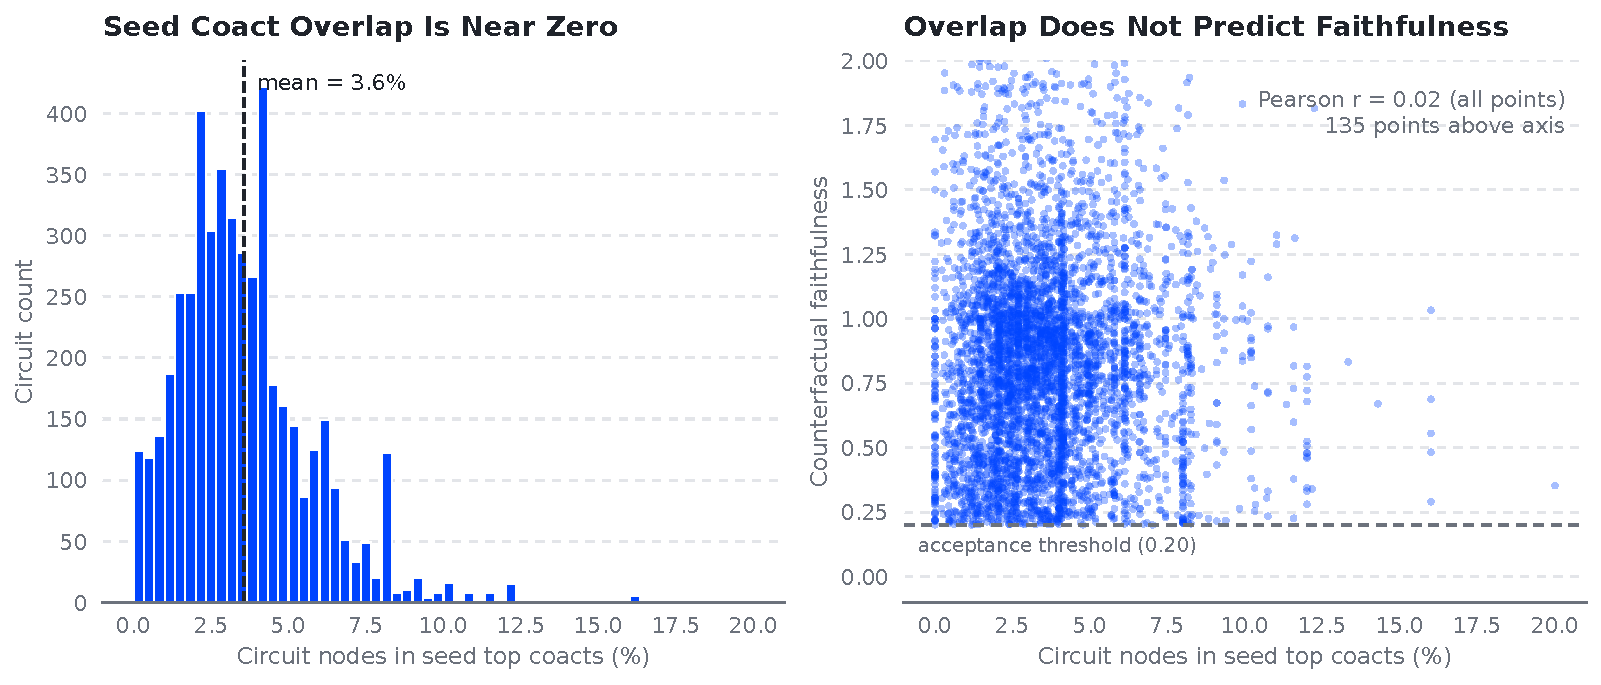
\includegraphics[width=\linewidth]{circuit-coact-overlap-paper.pdf}
\caption{Discovered dependencies are not co-activation neighbourhoods (\cref{sec:coact-results}).
Left: distribution of the percentage of each circuit's nodes that appear among its seed's top co-activation partners (mean 3.6\%).
Right: the same overlap against the circuit's counterfactual faithfulness (Pearson $r = 0.02$ over all points; 135 of 4{,}741 points lie above the truncated axis).
The dashed line marks the acceptance threshold (0.20), the minimum faithfulness an accepted circuit can have.
Statistics are over the 4{,}741 circuits with post-analysis co-activation metrics from the 7{,}525-circuit run.}
\label{fig:coact-overlap}
\end{figure}

\subsection{Metric Distributions Across Methods}
\label{app:eval-distributions}
% Demoted from the v1 body (Step 5): v1-grid data; the selection-effect
% observation is absorbed into the home-turf discussion in the body.

\begin{figure}
\centering
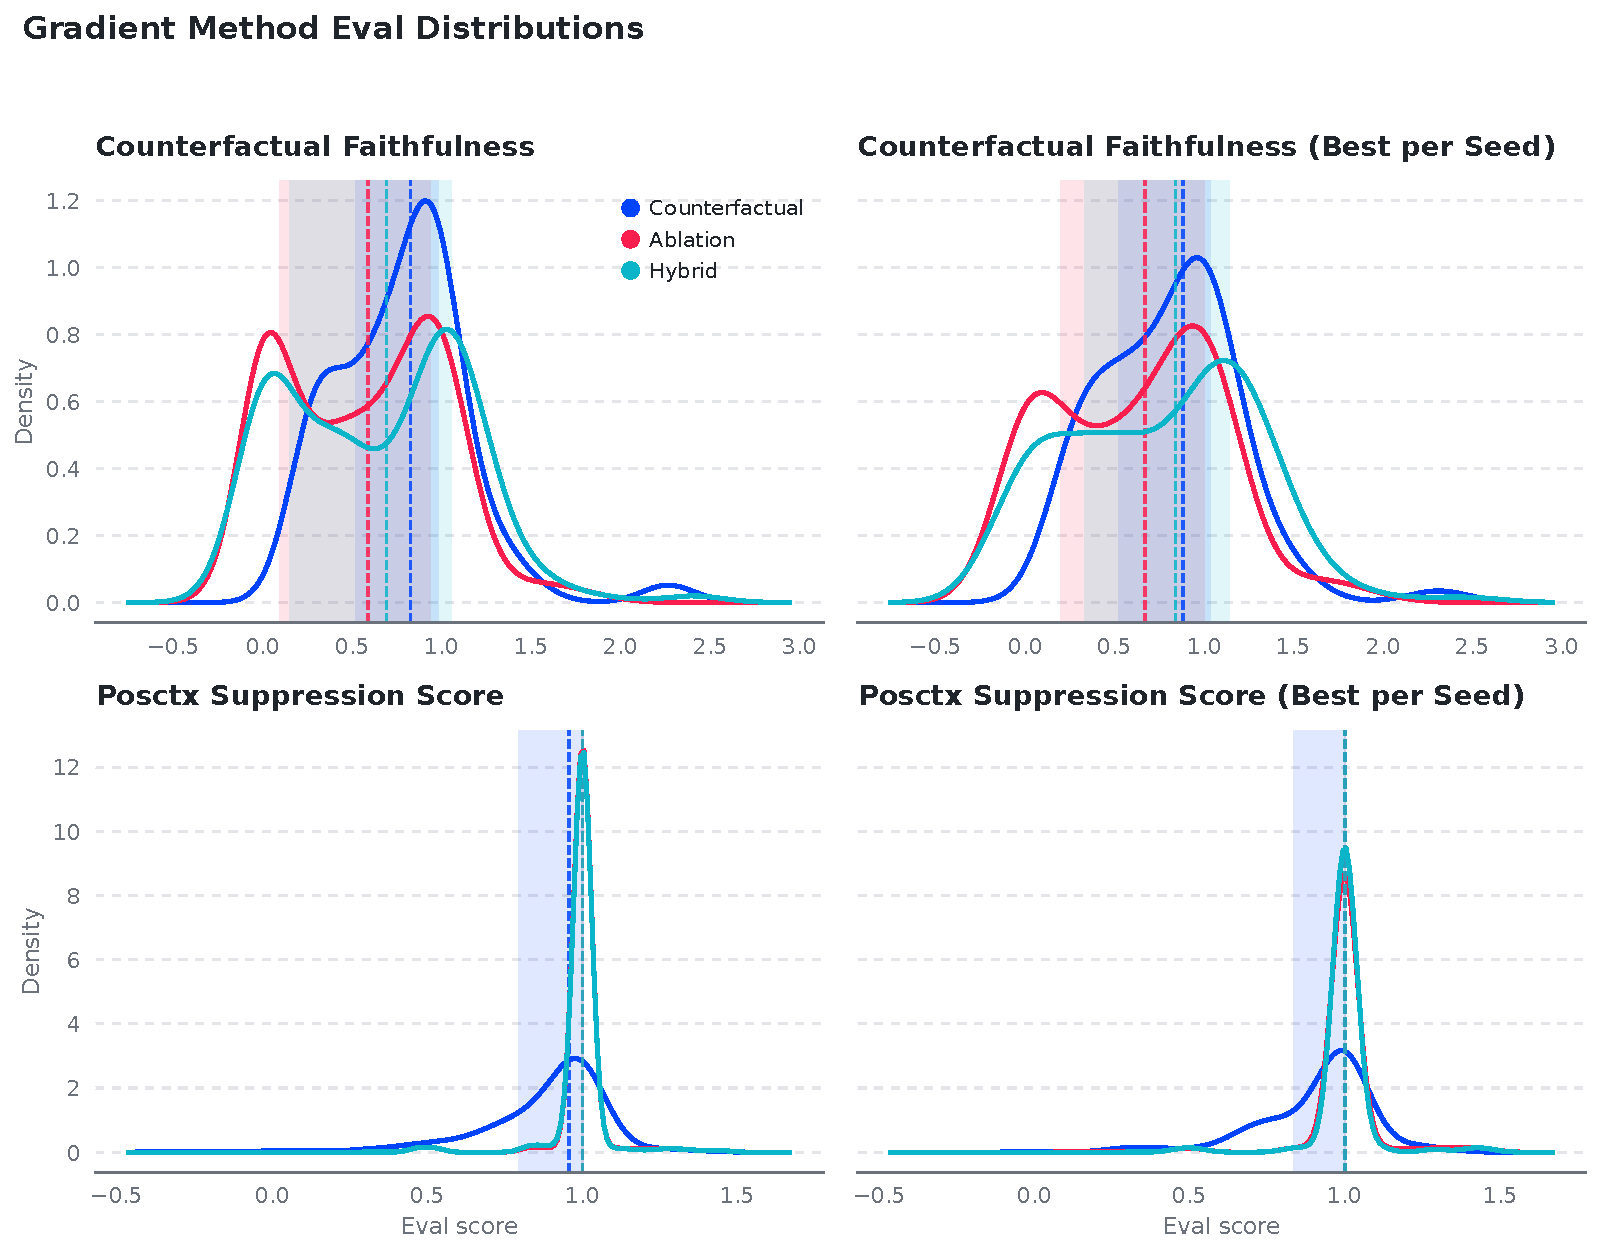
\includegraphics[width=\linewidth]{gradient-method-eval-distribution.pdf}
\caption{Kernel density estimates of counterfactual faithfulness (top row) and positive-context suppression score (bottom row) by discovery method.
Left column: all accepted circuits ($n = 857$).
Right column: each method's best accepted circuit per seed by counterfactual faithfulness --- at most one circuit from a seed's three negative-mode runs, an equal-budget comparison that does not reward a larger accepted pool (66, 117, and 117 seeds for counterfactual, ablation, and hybrid gradient respectively).
Dashed vertical lines mark medians; shaded regions span interquartile ranges.}
\label{fig:eval-distribution}
\end{figure}

The two rows of \cref{fig:eval-distribution} tell complementary stories.
On counterfactual faithfulness, counterfactual gradient produces a unimodal distribution with a sharp peak near 1.0 and a median of 0.82.
Ablation and hybrid gradient are bimodal --- a cluster near 0 and a second near 0.9 --- characteristic of methods that do not gate on faithfulness: some of their accepted circuits achieve it incidentally, while a non-trivial fraction are accepted on suppression grounds alone.
On suppression the picture reverses: ablation and hybrid produce near-singular distributions centred on 1.0, while counterfactual gradient spreads more widely below 1.0 with a median of 0.96.

No single method dominates both criteria, and each method looks strongest on the metric it gates on --- a selection effect inherent to comparing accepted-circuit populations; the body's home-turf effect (\cref{sec:method-comparison}) is the same phenomenon measured at the training objective rather than the acceptance gate.
The right column of \cref{fig:eval-distribution} controls for one such effect: restricting each method to its single best accepted circuit per seed --- every method received the same three negative-mode attempts per seed --- the qualitative pattern is unchanged, and ablation and hybrid gradient's low-faithfulness cluster shrinks but persists even at each seed's best attempt.

\subsection{Faithfulness by Circuit Size (v1 grid)}
\label{sec:size-curve}
% Demoted from the v1 body (Step 5): superseded there by the drivers/closure
% faithfulness-vs-size analysis (two-regime curve + depth-scaled core).

How much of a discovered ranking is needed, and what does more of it buy?
Following the circuit-size analysis of sparse feature circuits~\citep{marks2025sparse}, we re-run discovery on the same 128 seeds with the acceptance gates disabled --- so the curves are not conditioned on passing --- pruning off, random negatives, and the per-site candidate caps raised from 12 to 128 with attribution thresholds at zero, extending each seed's ranking well past the deployed circuit size.
Each circuit is truncated to its top-$m$ nodes per site and role for $m \in \{2, 4, 8, 12, 16, 32, 64, 128\}$, where $m = 12$ reproduces the deployed configuration, and every truncation is scored with the seed-intervention evaluation of \cref{sec:eval} on a per-seed context set shared across methods.
\cref{fig:size-curve} aggregates the resulting per-seed trajectories.

\begin{figure}
\centering
% MISSING FIGURE (lost in the 2026-07-22 teardown; figures/ was untracked).
% Regenerate from analysis-restyled/size-sweep data, or drop if this appendix
% is cut. Placeholder box keeps the build green meanwhile:
\fbox{\parbox[c][2.2in][c]{0.95\linewidth}{\centering\texttt{MISSING FIGURE: gradient-size-curve.pdf}\\ (to regenerate — see rewrite-tracker.md)}}
%\includegraphics[width=\linewidth]{gradient-size-curve.pdf}
\caption{Counterfactual faithfulness against circuit size, pre-gate.
Each seed's truncation trajectory is interpolated onto a common log-spaced node grid and aggregated pointwise across seeds (mean left, median right); grid positions covered by fewer than 25 seeds are dropped, which is where lines begin and end.
The dotted line marks $\phicf = 1$; values above it are intervention overshoot (\cref{sec:eval}).}
\label{fig:size-curve}
\end{figure}

Three observations.
First, faithfulness accumulates with circuit size throughout the sweep: no method plateaus below the overshoot line, and the deployed configuration (pre-gate mean $\phicf$ of 0.31, 0.56, and 0.62 for counterfactual, ablation, and hybrid gradient) sits well below what deeper rankings reach.
Second, size trades calibration for coverage: ablation gradient is the most node-efficient method at every size below roughly a thousand nodes, but its median crosses 1 near 1{,}000 nodes and hybrid's near 2{,}000 --- past that scale, added nodes increasingly overshoot the seed's positive-context mean rather than improve the reconstruction.
Third, counterfactual gradient's failures at the deployed size are budget-limited rather than fundamental: its pre-gate median faithfulness is 0 at $m = 12$ --- for over half the seeds the default circuit moves the seed not at all, consistent with its lower acceptance rate --- yet rises to 0.69 at $m = 128$ (median 4{,}350 nodes), so most seeds it fails at the deployed budget become reachable with a deeper per-site ranking.

\paragraph{Coverage across the SAE bank.}
\cref{fig:seed-breakdown} breaks the accepted grid circuits down by seed layer and seed component kind.
Every layer contributes accepted circuits (56--91 each), so the pipeline runs uniformly across the bank, and no strong layer trend emerges.
Scores are heterogeneous by component kind, however: residual-stream seeds achieve the highest faithfulness (median $\approx 0.97$), MLP-output seeds are intermediate ($\approx 0.41$), and attention-output seeds are hardest (median $\approx 0$).
This pooled view mixes methods and negative modes, so kind differences partly reflect which circuits each method's gate accepts; disentangling kind from method, and understanding why attention-output seeds resist counterfactual reconstruction, is left to future work.
The SAE quality measurements of \cref{app:sae-quality} narrow the search: attention SAEs are the bank's best reconstructors, so the failure is unlikely to be reconstruction fidelity --- their dead-latent structure and final-layer functional gap are the more plausible suspects.

\begin{figure}
\centering
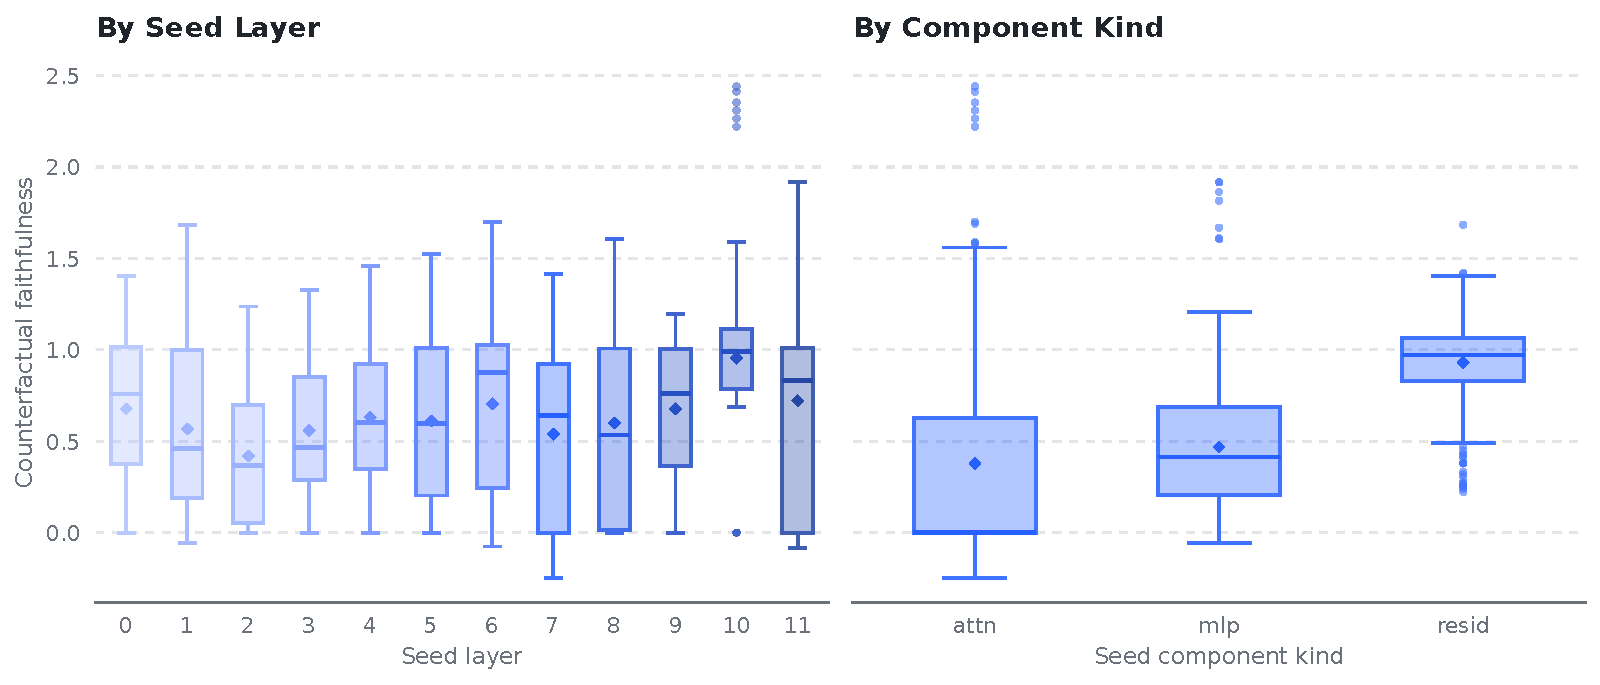
\includegraphics[width=\linewidth]{gradient-grid-seed-breakdown.pdf}
\caption{Counterfactual faithfulness of accepted grid circuits by seed layer (left) and seed component kind (right), pooled across methods and negative modes ($n = 857$).
Diamonds mark means; boxes span interquartile ranges.}
\label{fig:seed-breakdown}
\end{figure}

\paragraph{Circuit sizes.}
\cref{fig:circuit-size} shows accepted-circuit node counts by method and negative mode.
Counterfactual gradient returns the largest circuits (median 385 nodes), ablation gradient the smallest (median 193), with hybrid fusion between them (median 264); negative mode has little effect on size.

\begin{figure}
\centering
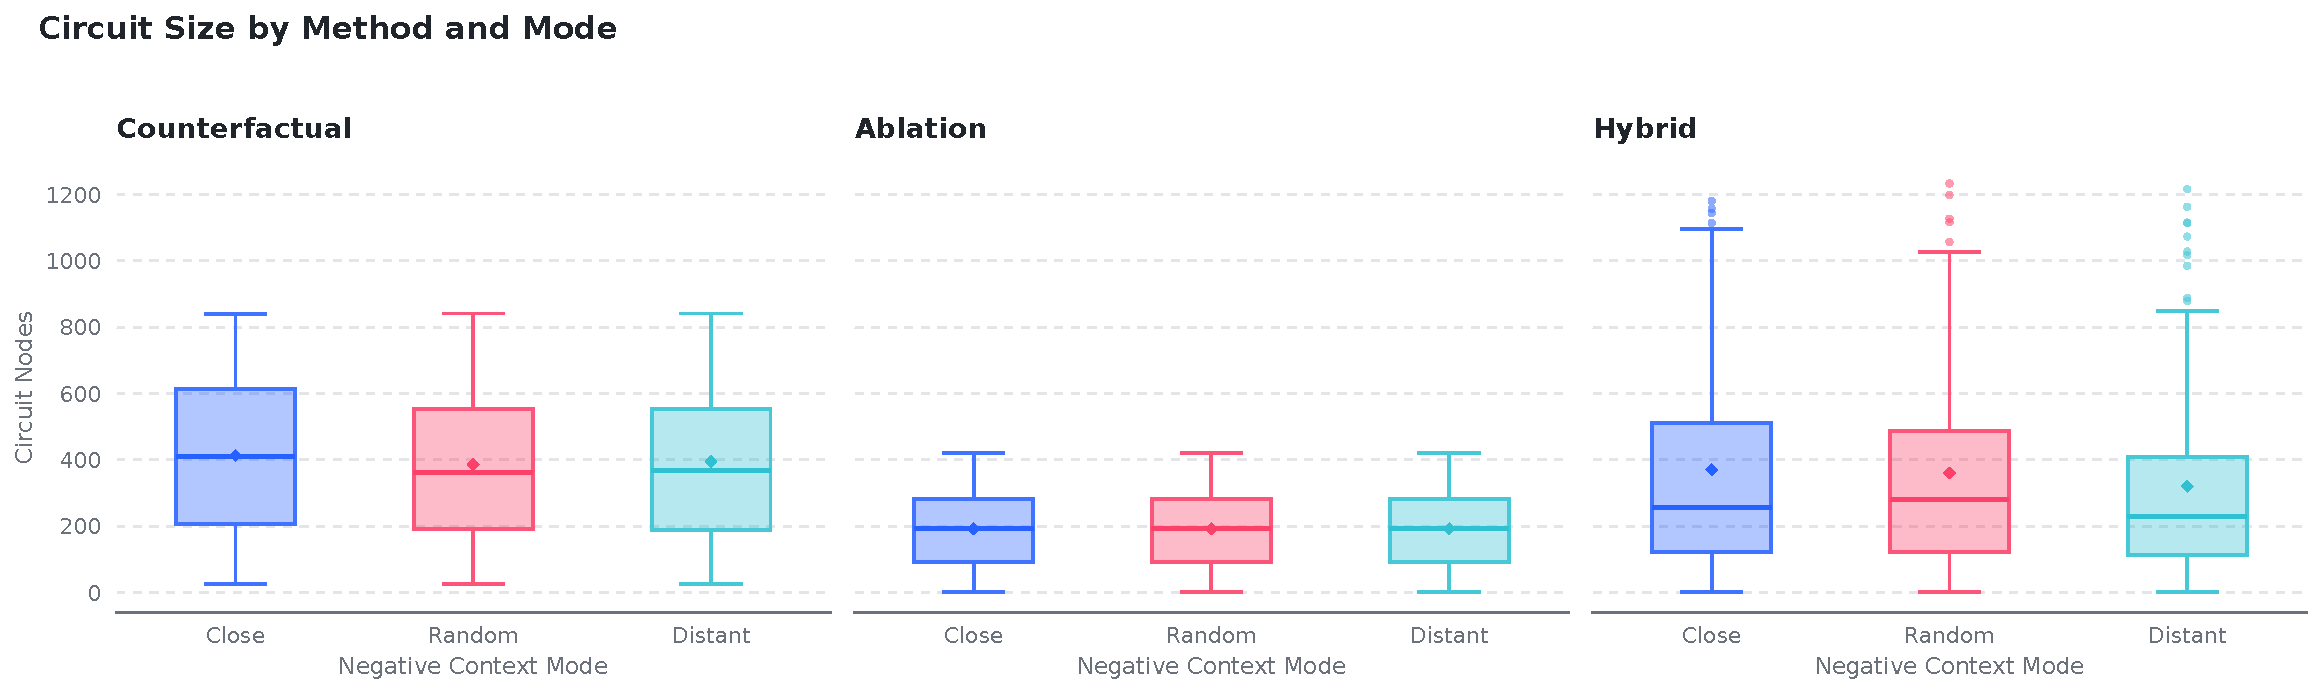
\includegraphics[width=\linewidth]{gradient-neg-mode-circuit-size-by-method.pdf}
\caption{Accepted circuit sizes (node counts) by discovery method and negative mode.}
\label{fig:circuit-size}
\end{figure}

\end{document}

